\section{Results} \label{results}

In this section, we first discuss the performance of the trained \ac{RF} and \ac{KNN} classifiers on the testing data set $D_S$ and use the latter to calculate the Bayesian probabilities
$P_M(I|{\bf A})$. Then we evaluate $P_M(I|{\bf A})$ on two independent data sets. The first set includes a population of simulated \ac{CBC} events that were injected in the real-time replay of
\ac{O3} data and was used for the \ac{LVK} \ac{MDC}~\cite{Chaudhary:2023vec}. The second set contains the confident \ac{LVK} \ac{O3} detections that are reported in \ac{LVK}'s \ac{GWTC3}
catalog~\cite{LIGOScientific:2021djp}.

\subsection{Performance on the \ac{O2} Testing Set}

We assess the performance of the classifiers by measuring the \ac{TPR} and the \ac{FPR} of the events in $D_S$. We present our findings as \ac{ROC} curves that illustrate how the \ac{TPR} varies
for various score thresholds as a function of the \ac{FPR}.

\begin{figure*}%[h]
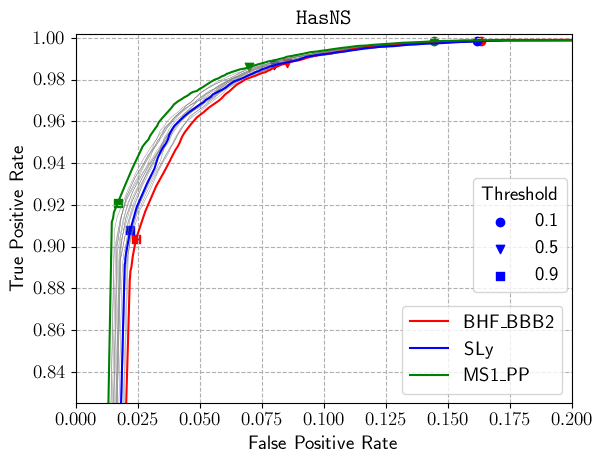
\includegraphics[width=0.45\linewidth]{roc_testing_KNN_NS}
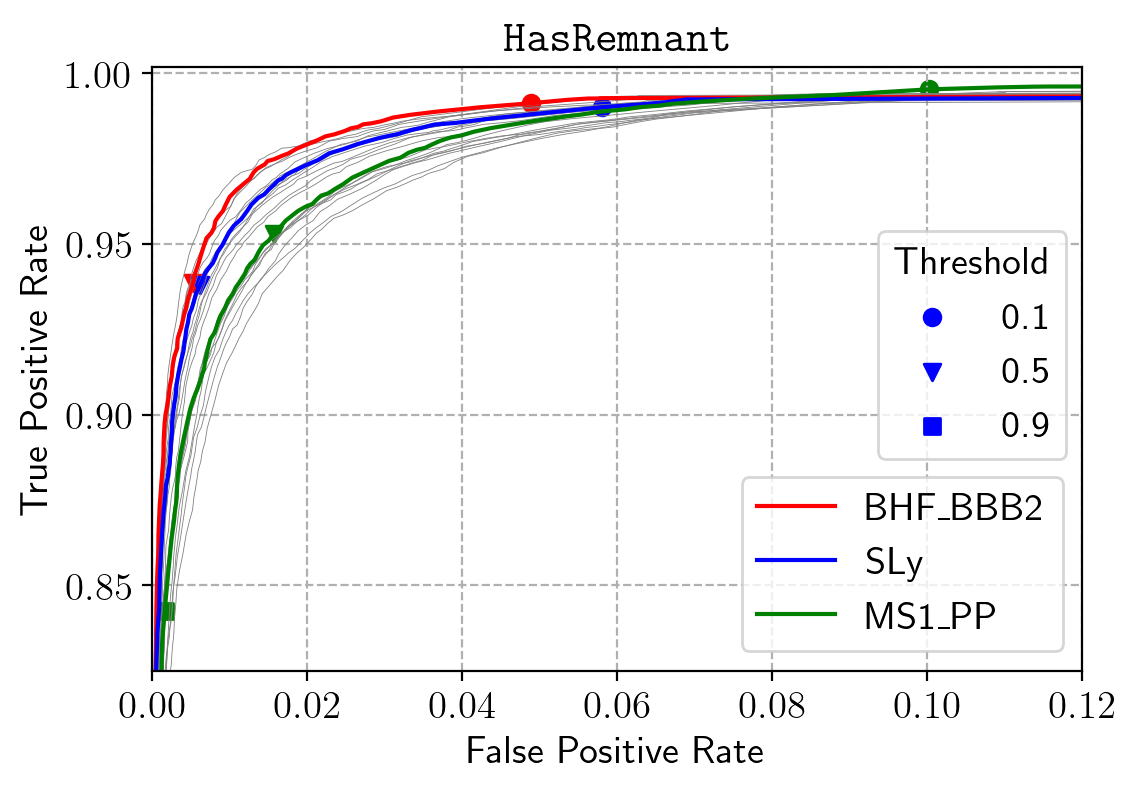
\includegraphics[width=0.45\linewidth]{roc_testing_KNN_REM}
\caption{\ac{ROC} curves obtained from the \ac{O2} testing data set $D_S$ for the \ac{KNN} classifier (left: \hasns, right: \hasrem). The curves for the 23 different \ac{EOS}s are displayed in
gray, with the curves for {\tt BHF\_BBB2}, {\tt MS1\_PP}, and {\tt SLy} highlighted in red, green, and blue, respectively. The circle, triangle, and square markers denote score thresholds of
$0.1$, $0.5$, and $0.9$, respectively.}
\label{fig:rocO2_KNN}
\end{figure*}

\begin{figure*}%[h]
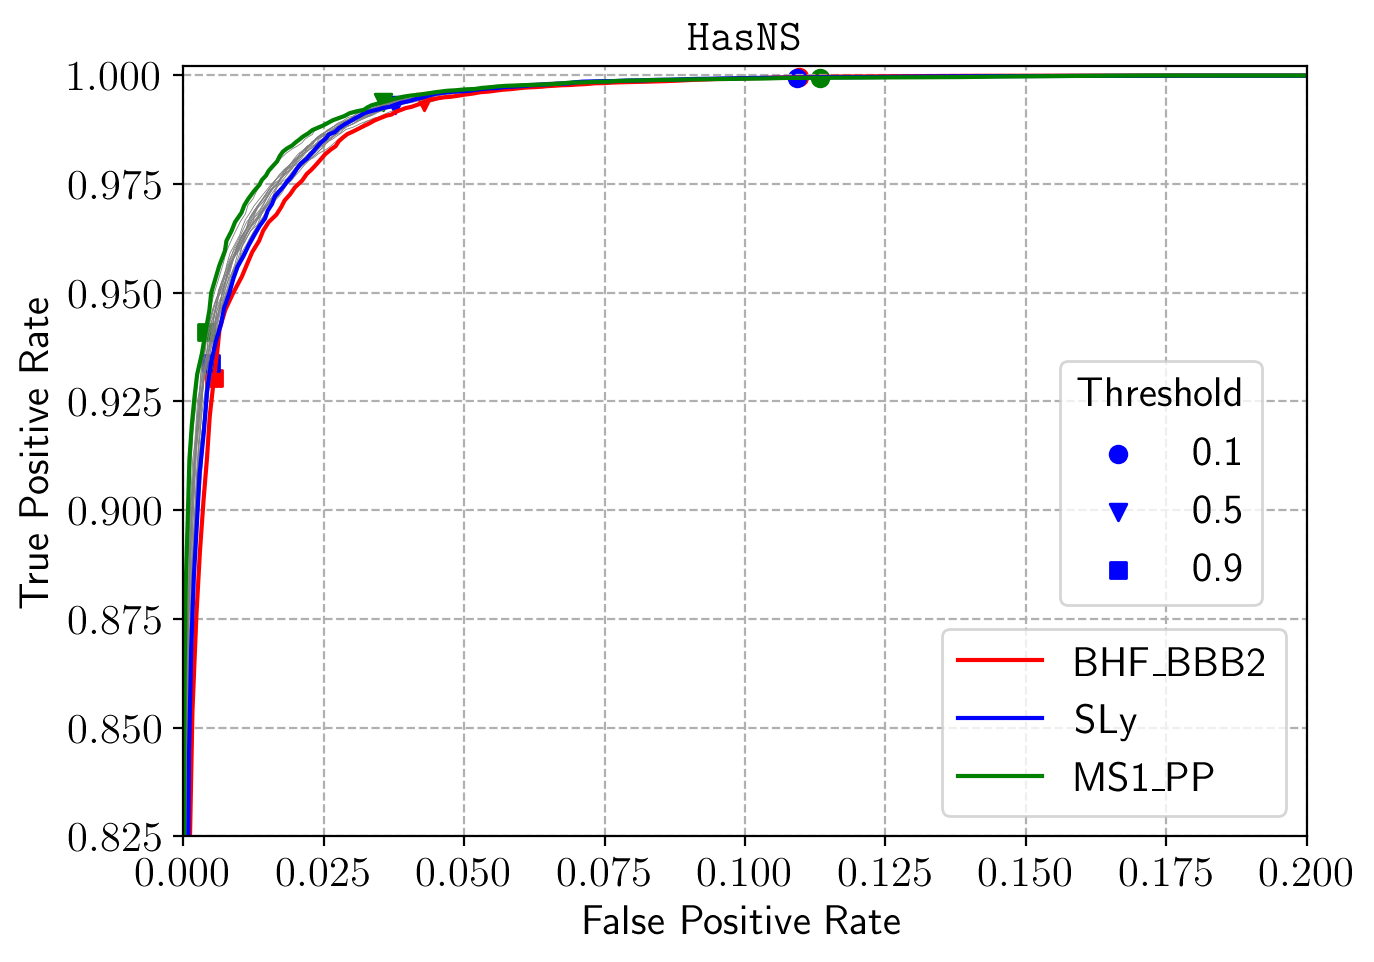
\includegraphics[width=0.47\linewidth]{roc_testing_RF_NS}
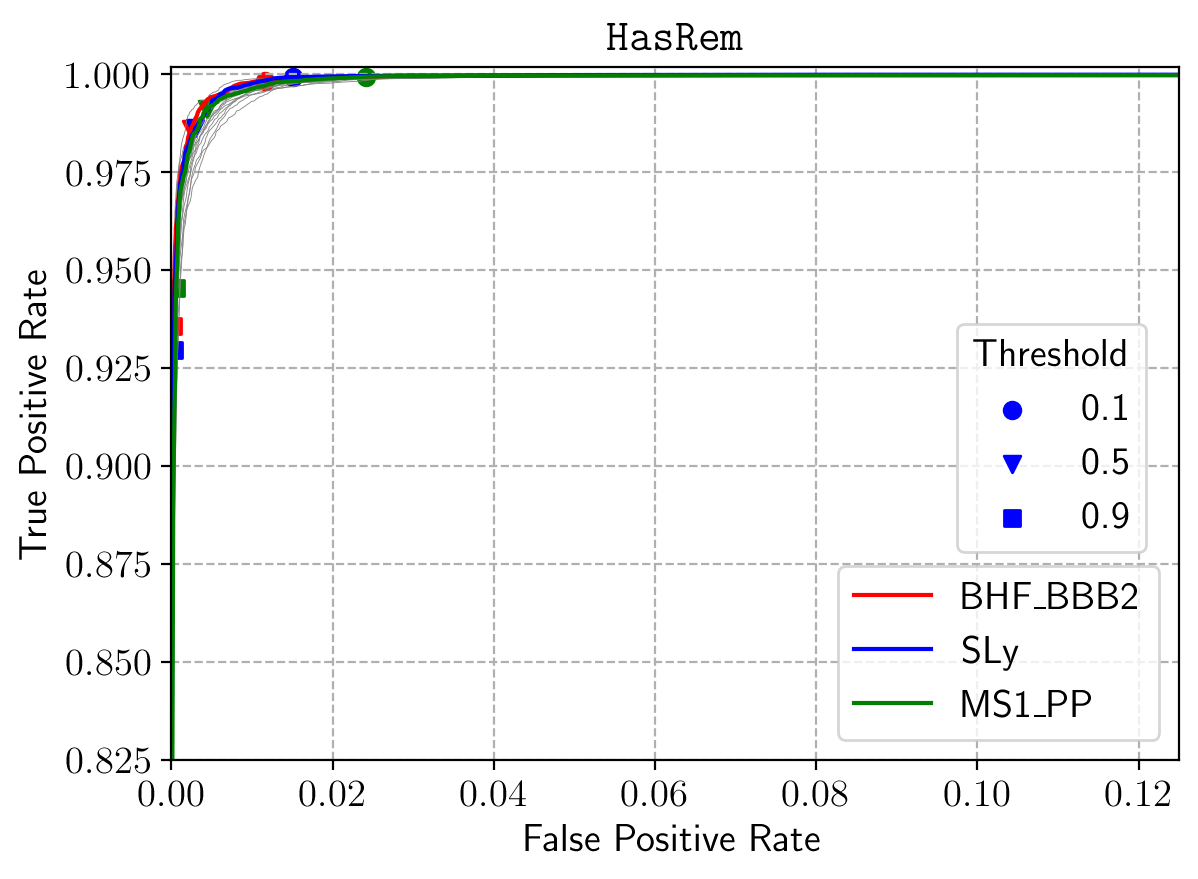
\includegraphics[width=0.45\linewidth]{roc_testing_RF_REM}
\caption{\ac{ROC} curves obtained from the \ac{O2} testing data set $D_S$ for the \ac{RF} classifier (left: \hasns, right: \hasrem). The curves for the 23 different \ac{EOS}s are displayed in
gray, with the curves for {\tt BHF\_BBB2}, {\tt MS1\_PP}, and {\tt SLy} highlighted in red, green, and blue, respectively. The circle, triangle, and square markers denote score thresholds of
$0.1$, $0.5$, and $0.9$, respectively.}
\label{fig:rocO2_RF}
\end{figure*}

The \hasns\ and \hasrem\ \ac{ROC} curves for the  \ac{KNN} algorithm are displayed in the left and right panels of Fig.~\ref{fig:rocO2_KNN}, respectively. Figure \ref{fig:rocO2_RF} displays the analogous curves for the \ac{RF} classifier. The \ac{ROC} curves for the 23 \ac{EOS} are plotted in grey, with three of them highlighted in color: {\tt BHF\_BBB2}, the \ac{EOS}
with the lowest maximum mass for the NS; {\tt MS1\_PP}, the \ac{EOS} with the largest maximum mass for the \ac{NS}; and {\tt SLy}, which allows for a maximum mass of $2.05 M_\odot$ and is
the standard \ac{EOS} used in \ac{LVK} low-latency investigations~\cite{Ghosh:2021eqv}. The markers denote different thresholds for the algorithm scores. 

The two classifiers perform consistently across all \ac{EOS}s. The \ac{TPR} for a score threshold of $0.5$ is around $0.99$ for both \hasns\ and \hasrem. A comparison of the
\hasns\ and \hasrem\ \ac{ROC} curves for each algorithm shows that the \ac{FPR} for \hasns\ is generally higher than the \ac{FPR} for \hasrem\ at a given threshold. Thus, the algorithms
typically do a better job in classifying \hasrem\ than \hasns. A separate comparison of the \ac{KNN} and \ac{RF} \ac{ROC} curves for \hasns\ and \hasrem\ shows that both algorithms perform
similarly on the O2 testing data set, with \ac{RF} producing slightly higher \ac{TPR} and lower \ac{FPR} than \ac{KNN} at a given threshold. 

\subsection{Bayesian Probabilities for the \ac{O3} Sets}

After the algorithms have been trained and tested, we compute the Bayesian probabilities defined in Sec.~\ref{bayesian_probs} in terms of their outcomes. Equations~\eqref{bayes-hasns} and \eqref{bayes-hasrem} must be assessed on a data set independent of the training data set, as stated in Sec.~\ref{bayesian_probs}. To do so, we employ $D_S$.

\begin{figure*}%[h]
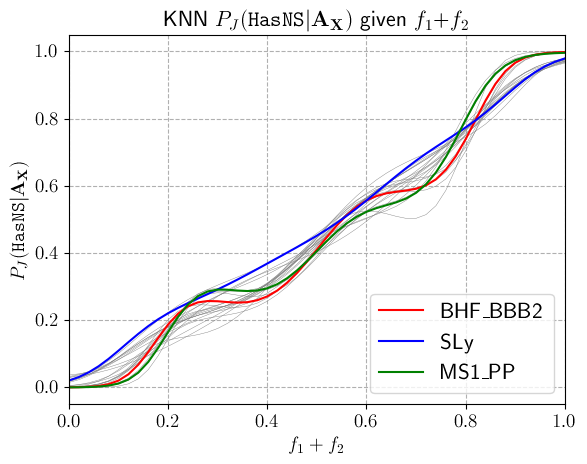
\includegraphics[width=0.45\linewidth]{KNN_3_eos_prob_plots_HasNS}
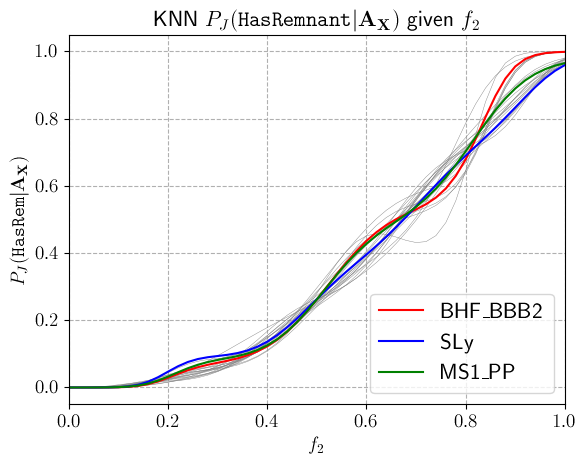
\includegraphics[width=0.45\linewidth]{KNN_3_eos_prob_plots_HasRem}
\caption{Left panel: \hasns\ Bayesian probability curves for the 23 \ac{EOS} as a function of the fraction of \ac{KNN} neighbors $f_1+f_2$. Right panel: \hasrem\ Bayesian probability curves as a function of the fraction of \ac{KNN} neighbors $f_2$. Curves for the {\tt BHF\_BBB2}, {\tt MS1\_PP}, and {\tt SLy} \ac{EOS}s are highlighted in red, green, and blue, respectively. The probabilities show an increasing trend as the fraction of neighbors increases. Non-monotonic fluctuations are due to the data set's finite size.}
\label{fig:bayesian_prob_fits_KNN}
\end{figure*}

\begin{figure*}%[h]
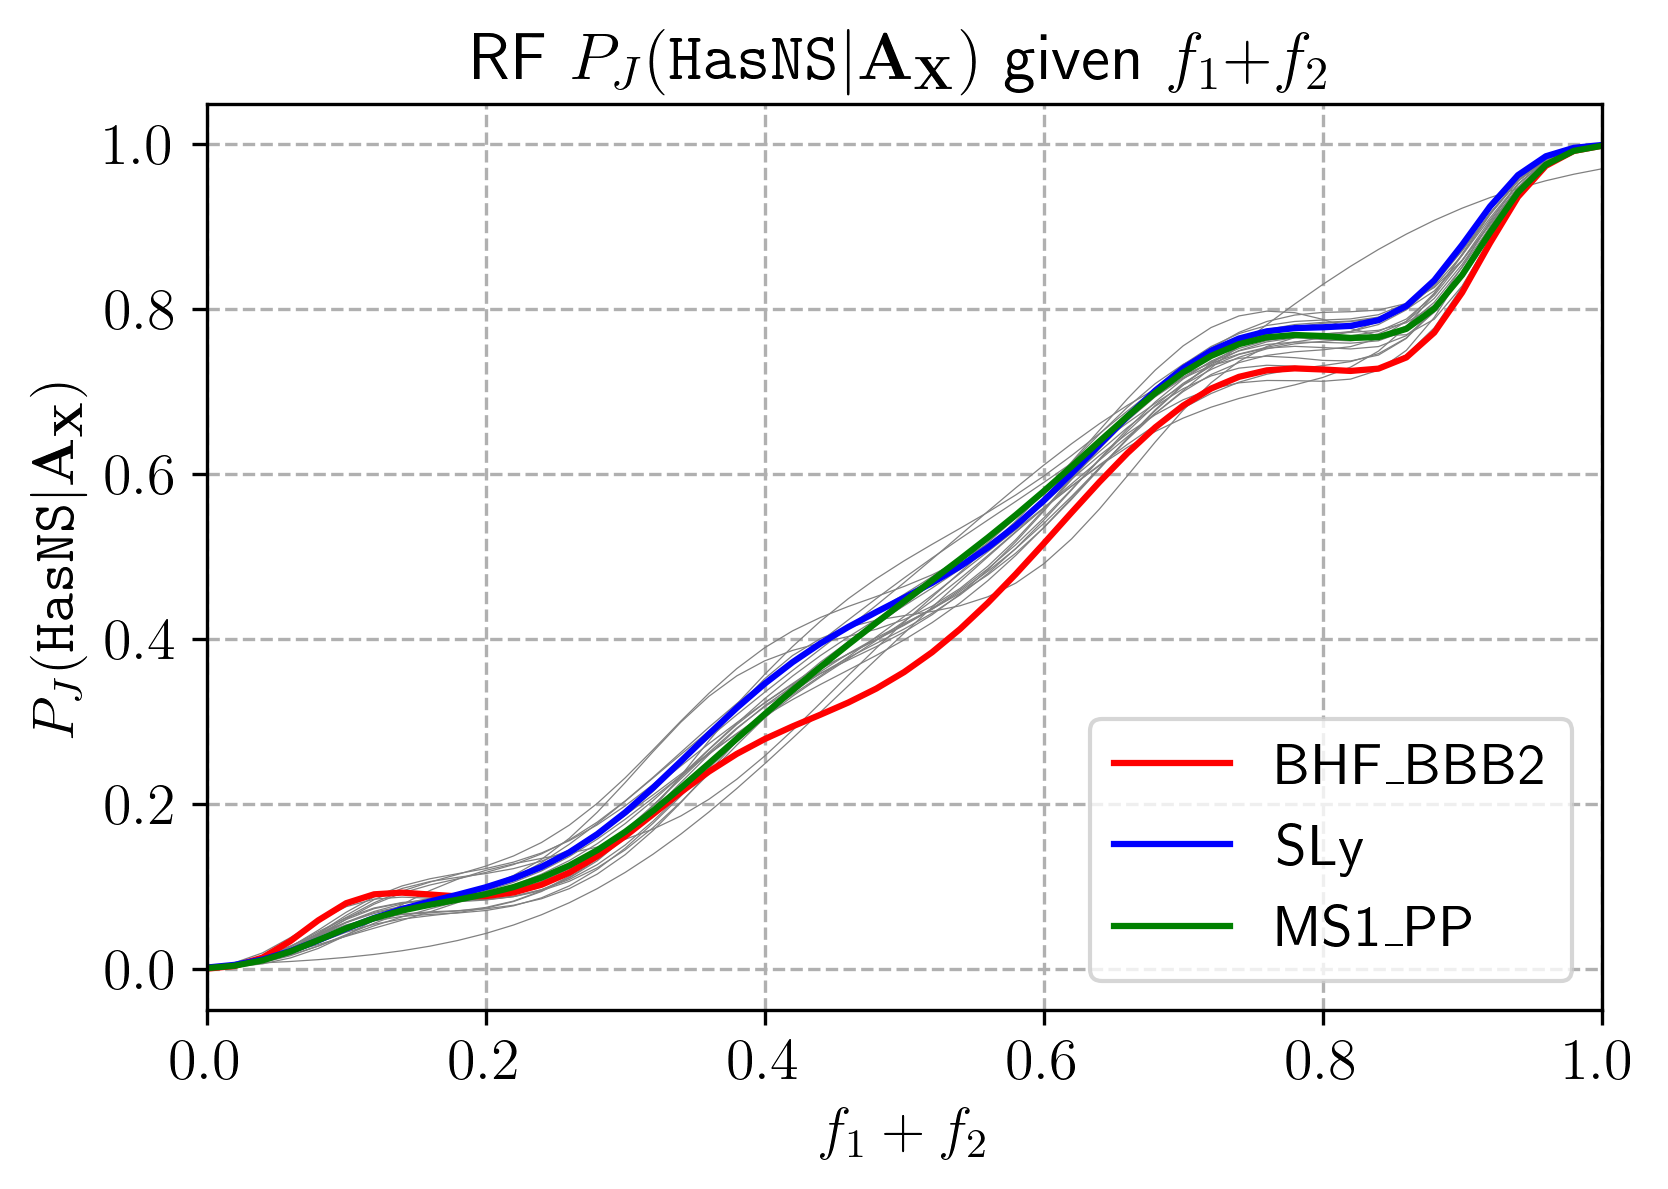
\includegraphics[width=0.45\linewidth]{RF_3_eos_prob_plots_HasNS}
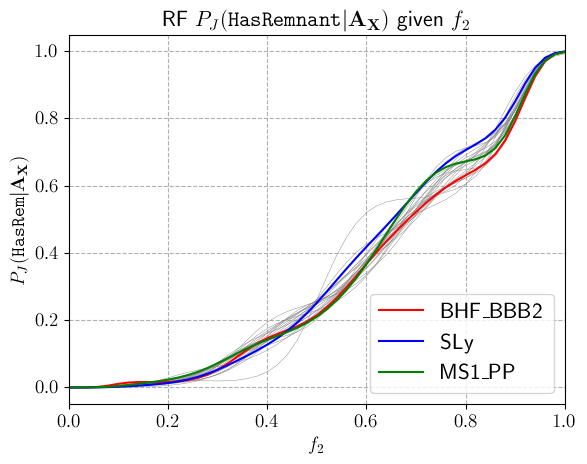
\includegraphics[width=0.45\linewidth]{RF_3_eos_prob_plots_HasRem}
\caption{Left panel: \hasns\ Bayesian probability curves for the 23 \ac{EOS} as a function of the fraction of \ac{RF} trees $f_1+f_2$. Right panel: \hasrem\ Bayesian probability curves for \hasrem\ as a function of the fraction of \ac{RF} Trees $f_2$. Curves for the {\tt BHF\_BBB2}, {\tt MS1\_PP}, and {\tt SLy} \ac{EOS}s are highlighted in red, green, and blue, respectively. The probabilities show an increasing trend as the fraction of trees increases.  Non-monotonic fluctuations are due to the data set's finite size.}
\label{fig:bayesian_prob_fits_RF}
\end{figure*}

Probability estimators for \ac{KNN} and \ac{RF} and each of the 23 \ac{EOS} are shown in Figs.~\ref{fig:bayesian_prob_fits_KNN} and~\ref{fig:bayesian_prob_fits_RF},
respectively. As expected, the \hasns\ and \hasrem\ probabilities increase with the fractions of \ac{KNN} neighbors (\ac{RF} trees). Local fluctuations in the probabilities are due to noise
arising from the finiteness of the data set. 

%The probability curves exhibit a sigmoid-like shapes that depend on the choice of the \ac{EOS}. Indeed, both show a slower
%increase of $P_J(\hasrem |\bf{A_X})$ for a low fraction $f_2$ compared to $P_J(\hasns |\bf{A_X})$. However, \ac{RF} shows a small plateau on the $P_J(\hasns |\bf{A_X})$ (and also on $P_J(\hasrem
%|\bf{A_X})$) for fractions of trees around $0.8$, which  \ac{KNN} does not reproduce. We highlight the same equations of state as in Figs.~\ref{fig:rocO2_KNN} and~\ref{fig:rocO2_RF}.

%\subsection{Performance on New Events}

The probabilities in Figs.~\ref{fig:bayesian_prob_fits_KNN} and~\ref{fig:bayesian_prob_fits_RF} can be tabulated and used to compute the marginalized probabilities $P_M(\hasns|{\bf A}_{\bf E})$
and $P_M(\hasrem|{\bf A}_{\bf E})$ as in Eq.~\eqref{bayes-marginalized}. To evaluate the method, we classify the events from the \ac{MDC} data set and compute the \ac{ROC} curves based on the
ground truth using Bayesian probability (rather than score) thresholds. The \ac{ROC} curves are shown in Figs.~\ref{fig:rocMDC_KNN} and \ref{fig:rocMDC_RF} for \ac{KNN} and \ac{RF},
respectively. In contrast to the \ac{O2} data set, the \ac{MDC} set contains outputs from four matched-filtering pipelines (GstLAL,  PyCBC~\cite{Usman:2015kfa}, SPIIR~\cite{Chu:2020pjv}, and
MBTA~\cite{Adams:2015ulm}). Therefore, we present separate \ac{ROC} curves for these pipelines. 

%Notice that the curves are very similar even though the algorithms were trained (and also the Bayesian probabilities were fitted) using exclusively GstLAL.

In the case of \hasns, \ac{KNN} yields a \ac{TPR} of 0.975 and an \ac{FPR} smaller than 0.2 for a probability threshold of 0.5 across all pipelines, with the exception of SPIIR. SPIIR's poorer
performance on \ac{EM} property classifications with the \ac{O3} \ac{MDC} set is a known effect that has been reported in other investigations~\cite{Chaudhary:2023vec}. In regard to \hasrem,
\ac{KNN} yields a \ac{TPR} around 0.975 and an \ac{FPR} slightly higher than 0.2 for the same threshold across all pipelines, with the exception of GstLAL. \ac{RF}'s results are similar to
\ac{KNN}'s results. The \ac{RF} \ac{ROC} curves for \hasns\ typically have steeper slopes than for \ac{KNN}, resulting in higher \ac{TPR} and lower \ac{FPR} at a given threshold. In the case of
\hasrem, \ac{RF} performs better than \ac{KNN} for GstLAL, but worse for other pipelines.

A few interesting results are worth mentioning.  On the \ac{MDC} set, both algorithms perform better for \hasns\ than \hasrem, whereas on the \ac{O2} set, the reverse is true (see Figs.~\ref{fig:rocO2_KNN} and~\ref{fig:rocO2_RF}). \ac{KNN} performs better than \ac{RF} on \hasrem, but does worse on \hasns. However, on events recovered by GstLAL, the pipeline on which the algorithms have been trained, both algorithms exhibit comparable (high) performance. This seems to indicate that when used with other pipelines, \ac{RF} is less flexible than \ac{KNN}. The conclusions provide more details about this and a possible explanation for this effect.
 
%\begin{comment}
%performs very well for \hasns achieving a true positive rate very close to
%unity with a very small false positive rate. We observe that SPIIR pipeline
%deviates from the good behaviour. For \hasrem the overall performance is
%slightly worse, getting higher false positive rate, but in turn all
%pipelines behave equally good. In Fig.~\ref{fig:rocMDC_RF} we showcase the results for \ac{RF}. As with \ac{KNN} the results are very good, with steep ROC curves. For \hasns spiir pipeline deviates less from the rest, getting higher positive rates for the same false positives than with \ac{KNN}. In the case of \hasrem the curves of the different pipelines behave a bit more differently from each other.
%\end{comment}

\begin{figure*}%[h]
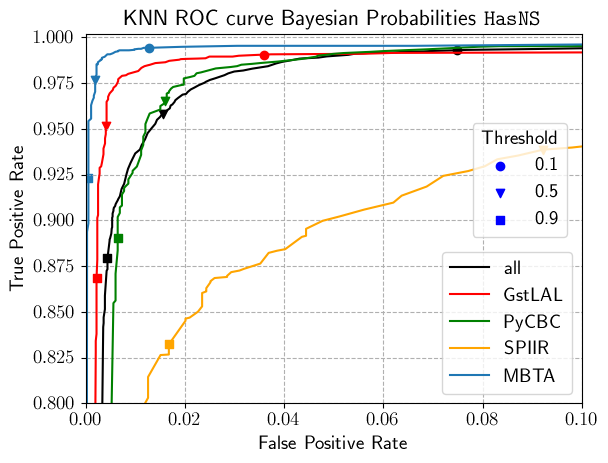
\includegraphics[width=0.45\linewidth]{roc_mdc_KNN_NS}
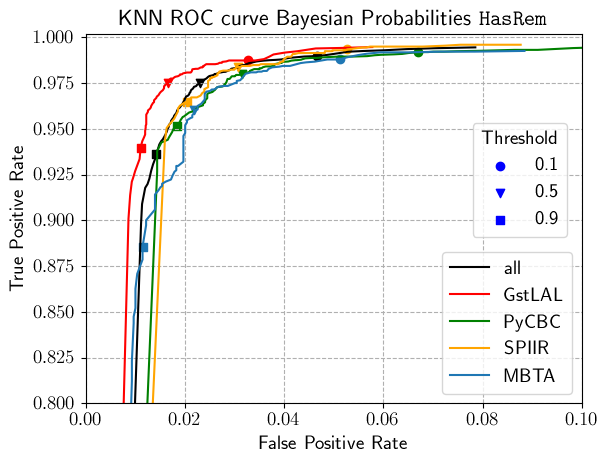
\includegraphics[width=0.45\linewidth]{roc_mdc_KNN_REM}
\caption{\ac{ROC} curves obtained from the \ac{O3} \ac{MDC} data set for the \ac{KNN} classifier (left: \hasns, right: \hasrem). The different \ac{LVK} matched-filtering pipelines are indicated by different colors (GstLAL: red; PyCBC: green; gold: SPIIR; blue: MBTA). The results for all pipelines are shown in black. The circle, triangle, and square markers denote probability thresholds of $0.1$, $0.5$, and $0.9$, respectively.}
\label{fig:rocMDC_KNN}
\end{figure*}


\begin{figure*}%[h]
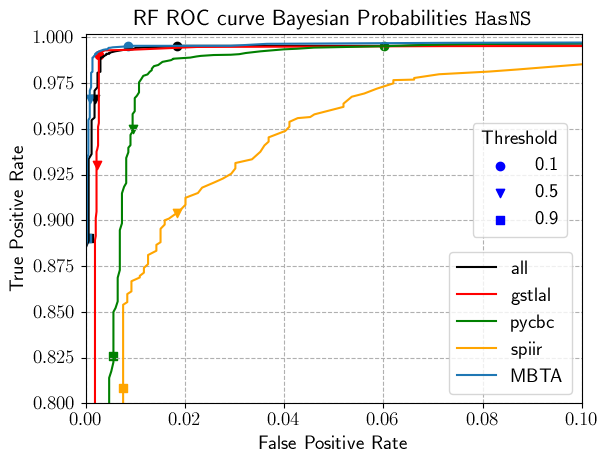
\includegraphics[width=0.45\linewidth]{roc_mdc_RF_NS}
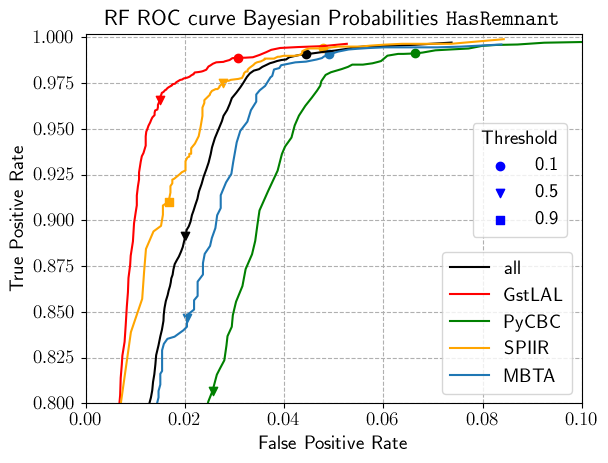
\includegraphics[width=0.45\linewidth]{roc_mdc_RF_REM}
\caption{\ac{ROC} curves obtained from the \ac{O3} \ac{MDC} data set for the \ac{RF} classifier (left: \hasns, right: \hasrem). The different \ac{LVK} matched-filtering pipelines are indicated by different colors (GstLAL: red; PyCBC: green; gold: SPIIR; blue: MBTA). The results for all pipelines are shown in black. The circle, triangle, and square markers denote probability thresholds of $0.1$, $0.5$, and $0.9$, respectively.}
\label{fig:rocMDC_RF}
\end{figure*}

Finally, we apply the method to derive Bayesian probabilities for the events in the \ac{LVK} \ac{GWTC3} catalog~\cite{LIGOScientific:2020ibl, LIGOScientific:2021djp}.  In
Table~\ref{tab:real_data_bayesian} we report the results for some of the most significant \ac{GWTC3} events, labeled with their event ID. The $P_M(\hasns |\bf{A_E})$ and $P_M(\hasrem |\bf{A_E})$ probabilities for GW170817 and GW190425, the two confirmed \ac{BNS}
detections~\cite{LIGOScientific:2020ibl,LIGOScientific:2021djp}, are $\sim 1$ as expected.  The probabilities for GW190426 and GW200115 (\ac{NSBH} mergers~\cite{LIGOScientific:2020ibl,
LIGOScientific:2021djp}) are $P_M(\hasns |{\bf{A_E}}) \sim 1$ and $P_M(\hasrem |{\bf{A_E}}) < 10^{-3}$. The two remaining significant events with non-zero probabilities are GW190814 and
GW190924. These events were reported as high mass-ratio BBH mergers~\cite{LIGOScientific:2020ibl, LIGOScientific:2021djp}. 

The fact that the system's component masses differ greatly from one another can be used to explain why $P_M(\hasns |\bf{A_E})$ for these events is not zero. In particular, the discrepancy
between \ac{RF} and \ac{KNN} for GW190814 can be understood from the different ways the two algorithms operate. \ac{RF} applies hard cuts on decision trees to evaluate its outcome. \ac{KNN}
looks at the fractions of neighbors surrounding the event. The detection pipeline returned a secondary mass compatible with an \ac{NS} for three of the 23 \ac{EOS}. However, since the region of
the parameter space close to the mass gap, i.e., the region between high \ac{NS} masses and low \ac{BH} masses, is not well covered in the \ac{O2} training data set, \ac{KNN} overestimates the
effect of the three \ac{EOS} predicting a secondary mass in the \ac{NS} region. 

\begin{table}[]
\begin{tabular}{c|cc|cc}
\hline
\multicolumn{1}{c|}{}      & \multicolumn{2}{c|}{$P_M(\hasns|{\bf A}_{\bf E})$}                                                & \multicolumn{2}{c}{$P_M(\hasrem|{\bf A}_{\bf E})$}                                                \\ \hline
\multicolumn{1}{c|}{event ID}   & \multicolumn{1}{c}{RF} & \multicolumn{1}{c}{KNN}  & \multicolumn{1}{c}{RF} & \multicolumn{1}{c}{KNN} \\ \hline
GW170817                                   & 0.998                   & 0.989                    & 0.997                   & 0.985                                  \\
GW190425                                   & 0.998                   & 0.989                    & 0.997                   & 0.985                            \\
GW190426                                   & 0.997                   & 0.985                    & $< 10^{-3}$             & $< 10^{-3}$                    \\
GW190814                                   & 0.042                   & 0.567                   & $< 10^{-3}$              & $< 10^{-3}$                      \\
GW190924                                   & 0.012                   & 0.054                   & $< 10^{-3}$              & $< 10^{-3}$                       \\               
GW200115                                   & 0.998                   & 0.989                   & $< 10^{-3}$              & $< 10^{-3}$                           \\
\hline
\end{tabular}
\caption{Bayesian probabilities of a few significant \ac{GW} events from the \ac{GWTC3} catalog. GW170817 and GW190425, GW190426 and GW200115, and GW190814 and GW190924 were determined to be \ac{BNS}, \ac{NSBH}, and \ac{BBH} mergers, respectively. The probability values in the table are rounded to three decimal figures.}
\label{tab:real_data_bayesian}
\end{table}

Figures~\ref{fig:param_sweep_KNN} and~\ref{fig:param_sweep_RF} show parameter sweeps in the space of the binary component masses for the \ac{KNN} and \ac{RF} Bayesian probabilities,
respectively. Different rows correspond to different values of the component spins. Both algorithms perform in a similar way for $P_M(\hasns |\bf{A_E})$. However, the parameter sweeps for
$P_M(\hasns |\bf{A_E})$ for \ac{KNN} are noisier than \ac{RF} for large primary masses. As was noted above, the \ac{KNN} algorithm operates by looking at the closest neighbors. If neighbors with
different label are present in the region of interest, the outcome is bound to be noisy. The \ac{RF} algorithm applies hard selection cuts to primary masses. This results in a more uniform
probability. Changes in spin seem to not significantly affect the outcome.  Similar behaviors for \ac{KNN} and \ac{RF} can also be observed in the case of $P_M(\hasrem |\bf{A_E})$. As expected
from the Foucart formula, $P_M(\hasrem |\bf{A_E})$ increases with the primary mass for large primary spins, and the region with $P_M(\hasrem |\bf{A_E}) \sim 1$ is included in the region where
$P_M(\hasns |\bf{A_E}) \sim 1$.

\begin{figure*}%[h]
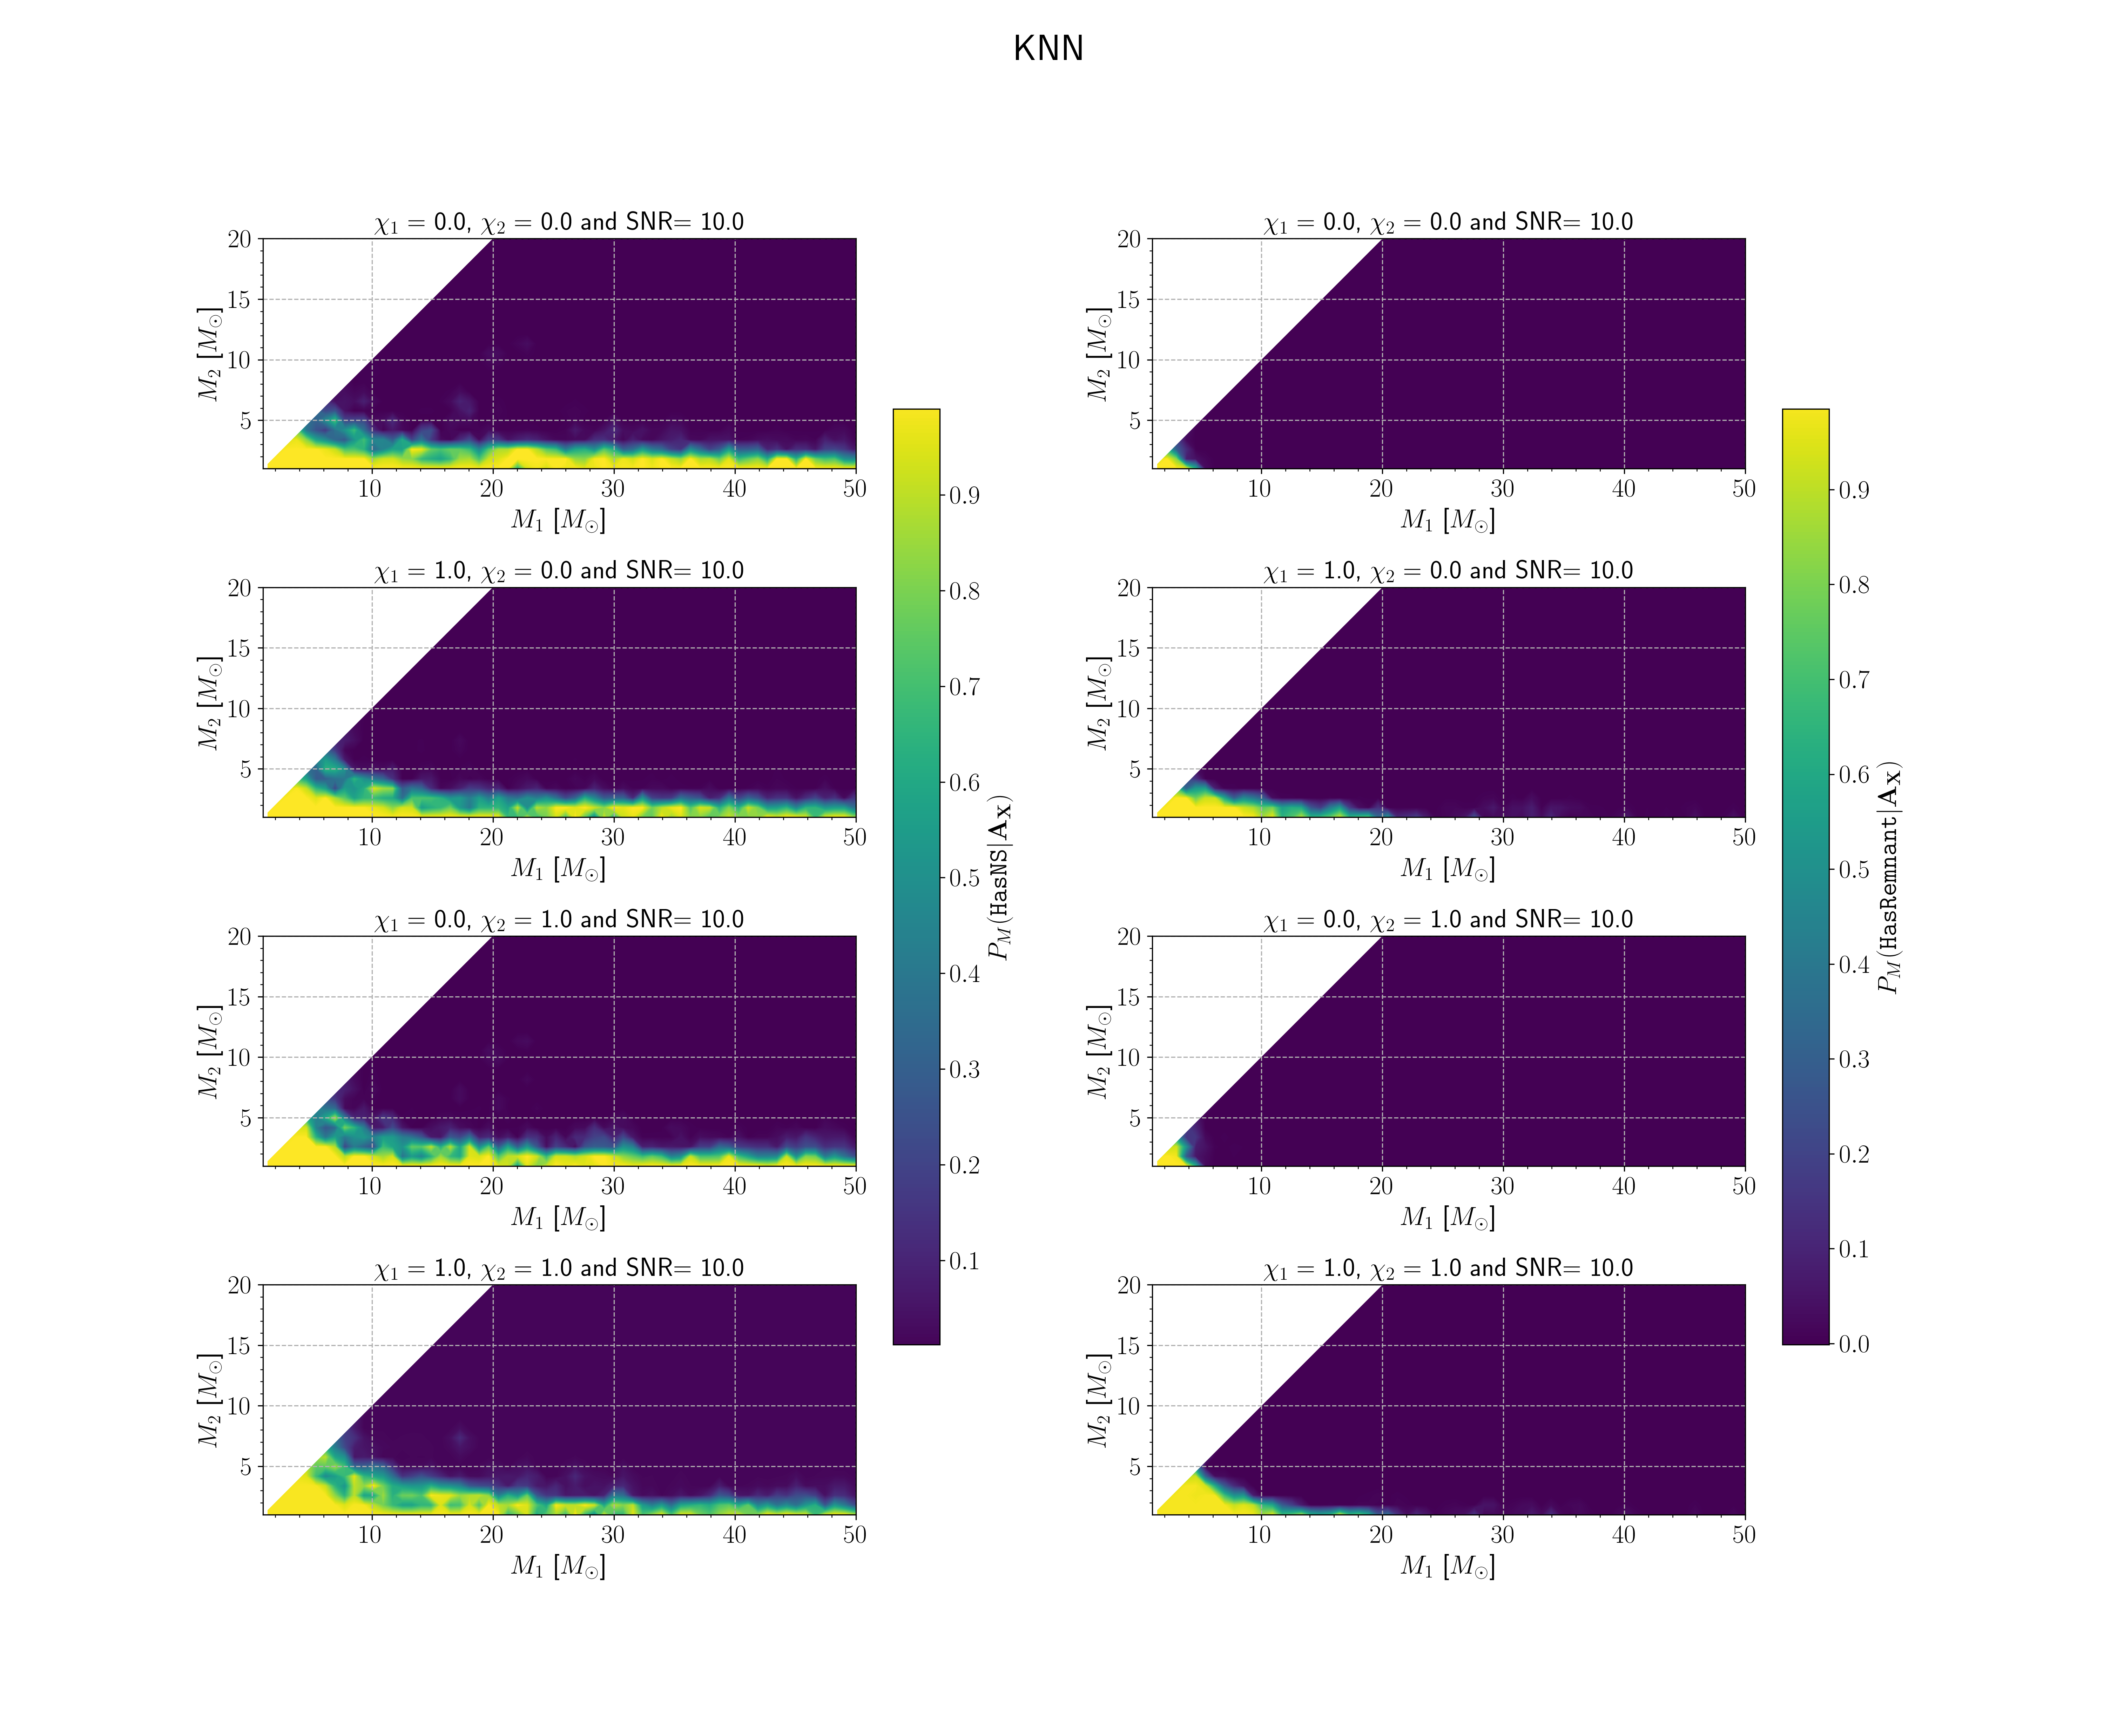
\includegraphics[width=0.9\linewidth]{KNN_parameter_sweep}
    \caption{Parameter sweeps for $P_M(\hasns |\bf{A_E})$ (left panels) and $P_M(\hasrem |\bf{A_E})$ (right panels) for the \ac{KNN} algorithm. $M_1$ and $M_2$ are the primary and secondary component masses of the binary. $\chi_1$ and $\chi_2$ are their effective spins. The \ac{SNR} is fixed to 10.}
\label{fig:param_sweep_KNN}
\end{figure*}

\begin{figure*}%[h]
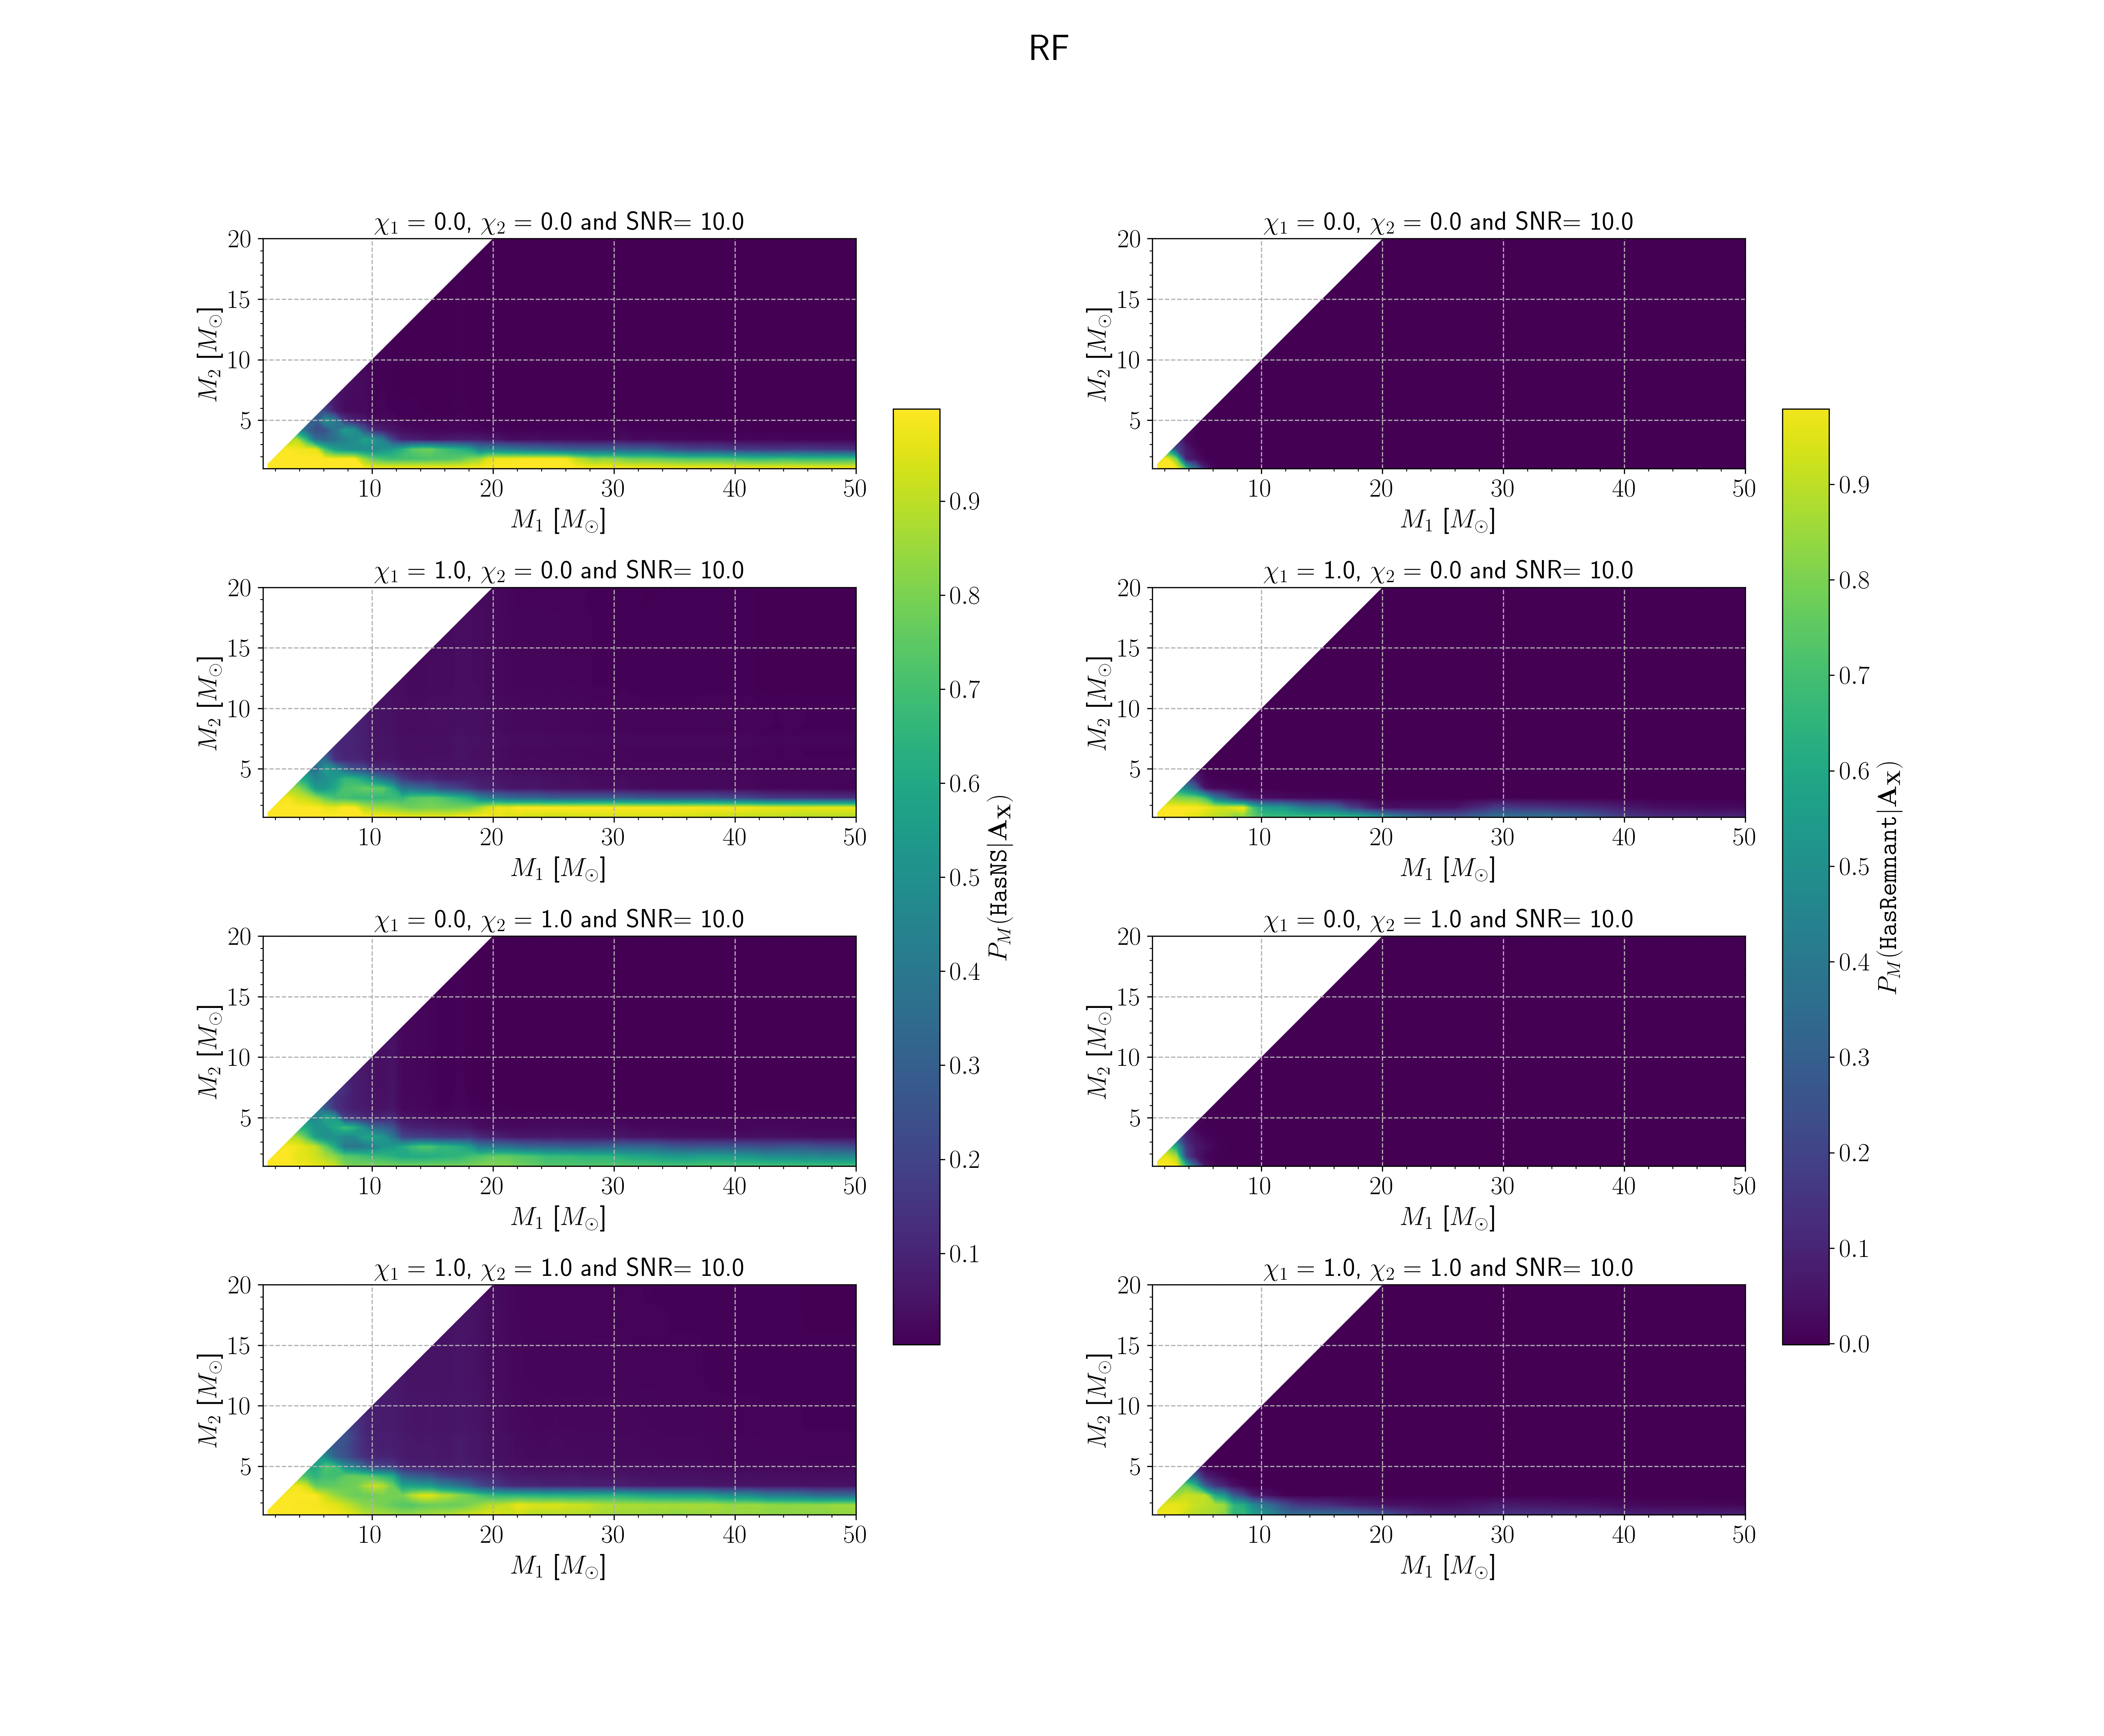
\includegraphics[width=0.9\linewidth]{RF_parameter_sweep}
    \caption{Parameter sweeps for $P_M(\hasns |\bf{A_E})$ (left panels) and $P_M(\hasrem |\bf{A_E})$ (right panels) for the \ac{RF} algorithm. $M_1$ and $M_2$ are the primary and secondary component masses of the binary. $\chi_1$ and $\chi_2$ are their effective spins. The \ac{SNR} is fixed to 10.}
\label{fig:param_sweep_RF}
\end{figure*}


%Here are the results for the methods:

%\subsection{KNN Results}

%\mmt{We are only using 5 features, the independent variables: 
%\begin{equation*}
	%\big[m_1,m_2,\chi_1,\chi_2, \rm{SNR}\big]\,.
%\end{equation*}}

\subsubsection{\mmt{Has NS}}
\mmt{The metric we use to compute the distance between neighbors is the \textit{Manhattan} metric (or the Minkowski's $L1$ distance),  which is the distance between two points measured along axes at right angles. Having $p_1(x_1,y_1)$ and $p_2(x_2,y_2)$ the distance will be}
\begin{equation}
	d = |x_1-x_2|+|y_1-y_2|\,.
\end{equation}

\mmt{Moreover, the points are weighted uniformly.  After applying cross-validation,  we get that the optimal number of neighbors is $K_{\rm NS} = 10$, with a mean score $\rm{s_m} = 0:9718355224352762$ and a testing score  $\rm{s_t} = 0.9723828730478842$.} 

%\begin{figure}
%    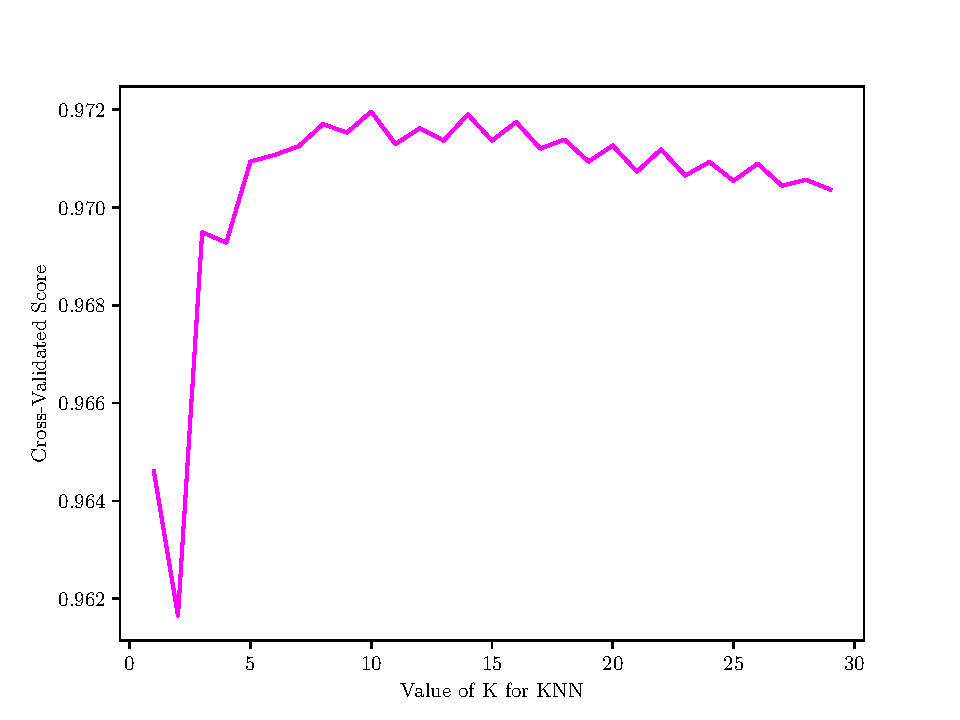
\includegraphics[width = 0.4\textwidth]{CrossValK.pdf}
%    \caption{Score of our KNN model as a function of the number of neighbors. We are considering \textit{HasNS}.}
%    \label{fig:crossvalK}
%\end{figure}
    
\begin{figure}
    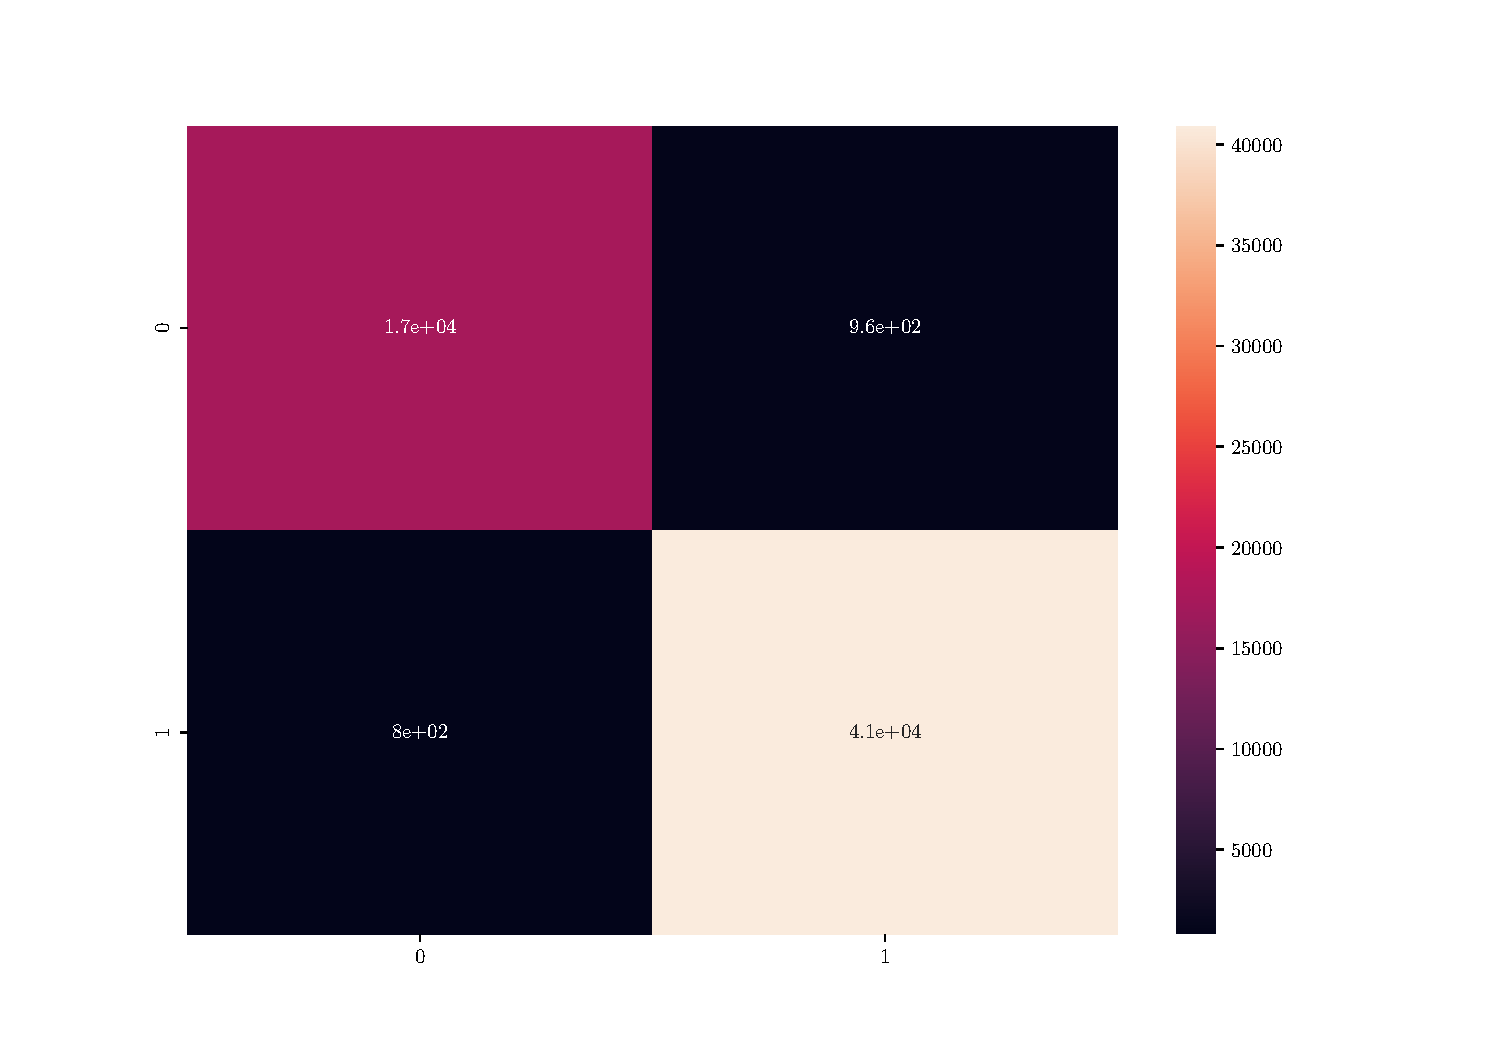
\includegraphics[width=0.45\textwidth]{figs/conf_matrix_NS.pdf}
    \caption{Confusion matrix for our model for \textit{HasNS}, using the independent recovered values. }
    \label{fig:confmat}
\end{figure}

\begin{figure}
    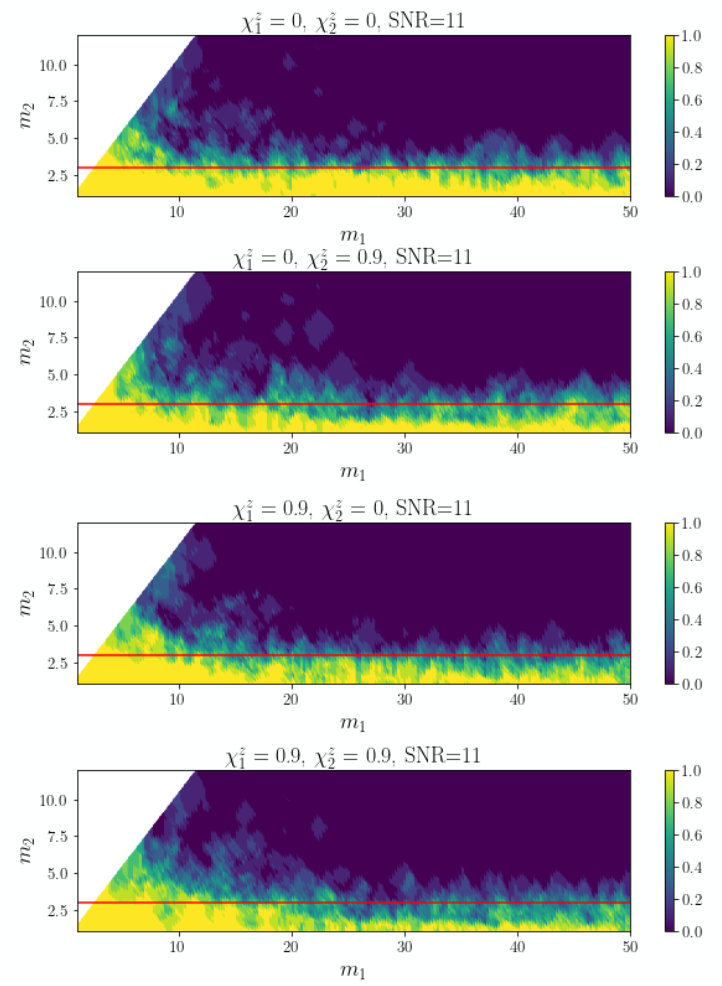
\includegraphics[width = 0.4\textwidth]{plot_fig4_chatt_spins.png}
  %   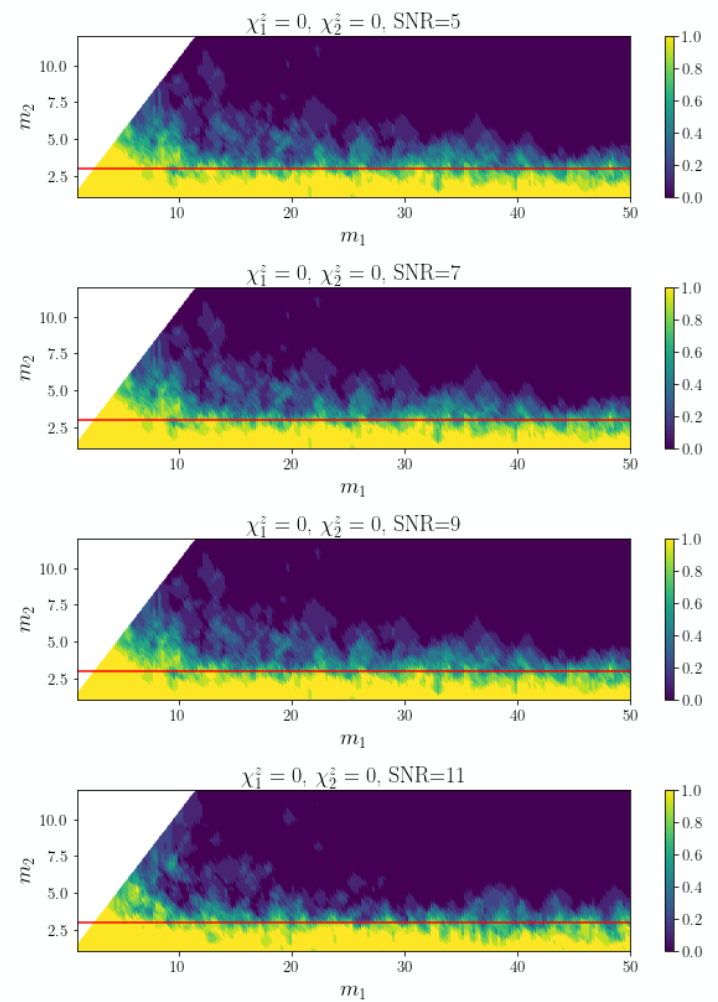
\includegraphics[width = 0.4\textwidth]{/Users/miquelmiravet/Projects/IPAM_LA/ML_group/IPAM2021_ML/algo/classy_KNN/PLOTS_KNN/NS_set/plots_miq/plot_fig4_chatt_snr.png}
    \caption{Probability of having a remnant as a function of the values of the masses. The different panels show the results for different spins. The solid red line depicts the threshold mass for $m_2$.}
    \label{fig:m1m2}
\end{figure}

\begin{figure}
	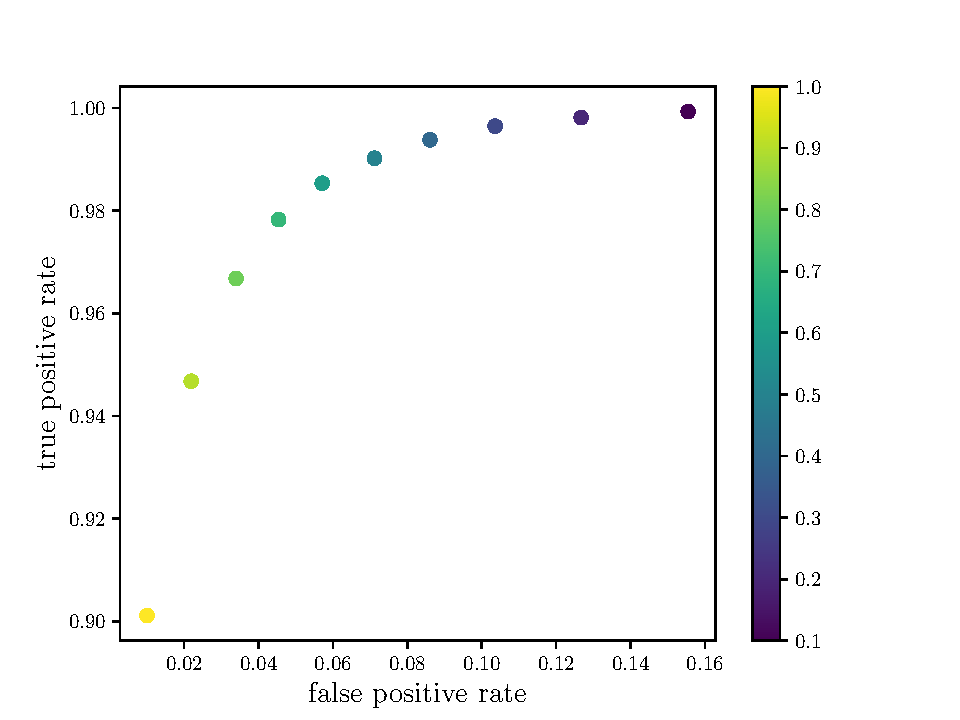
\includegraphics[width =0.4\textwidth]{ROCplot.pdf}
    \caption{Relation of the true and false positive rates as a function of the threshold applied to make the decision between having or not having a remnant. }
    \label{fig:roc}
\end{figure}

\mmt{In Fig.~\ref{fig:crossvalK} you can find how the mean score changes with the number of neighbors of the algorithm.  The confusion matrix appears in Fig.~\ref{fig:confmat}, the probability as a function of $m_1$ and $m_2$  is shown in Figs.~\ref{fig:m1m2}, and the true and false positive rates in terms of the threshold probability appear in Fig.~\ref{fig:roc}.}


 %plots and comments
%\subsection{RF Results}

We apply crossvalidation in the number of trees and depth of the forests for the 23 EoS, fixing the information gain criteria to \texttt{entropy}. We also save the second best option for comparison, and save both forests for each EoS in order to compare the file size. As the goal is to provide a model that can run in a low latency pipeline the amount of memory it can take is limited, even more when there will be 23 different model for the EoS generalization.

In table \ref{tab:RFcross} we present a summary of best and second best hyperparameters found in the crossvalidation for each EoS, along the memory the model occupies and the difference in the score. As we can see, usually a forest with many trees has a second best option with far less that is lighter in memory and achieves a similar performance. The optimum maximum depth is always 15. Also the score achieved for every EoS is similar, and so we check that our accuracy is not NS model dependent.

\begin{table*}[h]
\centering
\begin{tabular}{@{}lcccccccc@{}}
\toprule
                                & \multicolumn{4}{c}{Best}                                & \multicolumn{4}{c}{Second best}                            \\ \midrule
\multicolumn{1}{|l|}{EOS}       & Trees & Depth & Size(MB)    & \multicolumn{1}{c|}{Score}      & Trees & Depth & Size(MB)    & \multicolumn{1}{c|}{$\Delta$score} \\ \midrule
\multicolumn{1}{|l|}{APR4\_BB}  & 300   & 15    & 94.7  & \multicolumn{1}{c|}{0.9683018}  & 50    & 15    & 15.7  & \multicolumn{1}{c|}{3.35e-5}       \\ \midrule
\multicolumn{1}{|l|}{BHF\_BBB2} & 80    & 15    & 24.4  & \multicolumn{1}{c|}{0.9685127}  & 300   & 15    & 91.6  & \multicolumn{1}{c|}{5.16e-5}       \\ \midrule
\multicolumn{1}{|l|}{H4}        & 80    & 15    & 29.6  & \multicolumn{1}{c|}{0.9618587}  & 300   & 15    & 111.4 & \multicolumn{1}{c|}{1.19e-4}       \\ \midrule
\multicolumn{1}{|l|}{HQC18}     & 300   & 15    & 93.7  & \multicolumn{1}{c|}{0.9673755}  & 100   & 15    & 31.3  & \multicolumn{1}{c|}{3.06e-4}       \\ \midrule
\multicolumn{1}{|l|}{KDE0V}     & 300   & 15    & 92.0  & \multicolumn{1}{c|}{0.9673295}  & 80    & 15    & 24.5  & \multicolumn{1}{c|}{2.06e-4}       \\ \midrule
\multicolumn{1}{|l|}{KDE0V1}    & 100   & 15    & 30.9  & \multicolumn{1}{c|}{0.96704954} & 80    & 15    & 24.5  & \multicolumn{1}{c|}{3.43e-5}       \\ \midrule
\multicolumn{1}{|l|}{MPA1}      & 80    & 15    & 27.2  & \multicolumn{1}{c|}{0.96601225} & 300   & 15    & 102.1 & \multicolumn{1}{c|}{8.19e-5}       \\ \midrule
\multicolumn{1}{|l|}{MS1\_PP}   & 300   & 15    & 113.5 & \multicolumn{1}{c|}{0.96563534} & 80    & 15    & 30.2  & \multicolumn{1}{c|}{1.15e-4}       \\ \midrule
\multicolumn{1}{|l|}{MS1B\_PP}  & 300   & 15    & 114.2 & \multicolumn{1}{c|}{0.96555340} & 100   & 15    & 38.0  & \multicolumn{1}{c|}{1.97e-4}       \\ \midrule
\multicolumn{1}{|l|}{RS}        & 300   & 15    & 103.8 & \multicolumn{1}{c|}{0.96447350} & 80    & 15    & 27.6  & \multicolumn{1}{c|}{2.36e-4}       \\ \midrule
\multicolumn{1}{|l|}{SK255}     & 300   & 15    & 105.8 & \multicolumn{1}{c|}{0.96472405} & 100   & 15    & 35.5  & \multicolumn{1}{c|}{3.69e-4}       \\ \midrule
\multicolumn{1}{|l|}{SK272}     & 300   & 15    & 109.0 & \multicolumn{1}{c|}{0.96401816} & 100   & 15    & 36.4  & \multicolumn{1}{c|}{1.99e-4}       \\ \midrule
\multicolumn{1}{|l|}{SKI2}      & 50    & 15    & 18.8  & \multicolumn{1}{c|}{0.96242338} & 300   & 15    & 112.8 & \multicolumn{1}{c|}{8.37e-5}       \\ \midrule
\multicolumn{1}{|l|}{SKI3}      & 50    & 15    & 19.0  & \multicolumn{1}{c|}{0.96174537} & 100   & 15    & 38.1  & \multicolumn{1}{c|}{6.62e-5}       \\ \midrule
\multicolumn{1}{|l|}{SKI4}      & 300   & 15    & 100.6 & \multicolumn{1}{c|}{0.96598969} & 30    & 15    & 9.8   & \multicolumn{1}{c|}{8.37e-5}       \\ \midrule
\multicolumn{1}{|l|}{SKI5}      & 100   & 15    & 38.2  & \multicolumn{1}{c|}{0.96343381} & 80    & 15    & 30.4  & \multicolumn{1}{c|}{1.16e-4}       \\ \midrule
\multicolumn{1}{|l|}{SKI6}      & 300   & 15    & 101.7 & \multicolumn{1}{c|}{0.96586928} & 30    & 15    & 10.0  & \multicolumn{1}{c|}{2.17e-4}       \\ \midrule
\multicolumn{1}{|l|}{SKMP}      & 300   & 15    & 100.2 & \multicolumn{1}{c|}{0.96544567} & 80    & 15    & 26.9  & \multicolumn{1}{c|}{1.69e-4}       \\ \midrule
\multicolumn{1}{|l|}{SKOP}      & 100   & 15    & 32.3  & \multicolumn{1}{c|}{0.96610459} & 300   & 15    & 96.2  & \multicolumn{1}{c|}{6.85e-5}       \\ \midrule
\multicolumn{1}{|l|}{SLy}       & 80    & 15    & 25.3  & \multicolumn{1}{c|}{0.96728884} & 300   & 15    & 95.2  & \multicolumn{1}{c|}{8.49e-5}       \\ \midrule
\multicolumn{1}{|l|}{SLY2}      & 100   & 15    & 31.8  & \multicolumn{1}{c|}{0.96745868} & 80    & 15    & 25.4  & \multicolumn{1}{c|}{2.38e-4}       \\ \midrule
\multicolumn{1}{|l|}{SLY9}      & 300   & 15    & 101.6 & \multicolumn{1}{c|}{0.96605993} & 100   & 15    & 34.1  & \multicolumn{1}{c|}{1.51e-4}       \\ \midrule
SLY230A                         & 300   & 15    & 95.5  & 0.96714915                      & 100   & 15    & 31.9  & 2.53e-4                            \\ \bottomrule
\end{tabular}
\caption{Comparison of the best and second best RF models obtained during crossvalidation for all EoS. We show the file size in MB of the forest, and the difference in score between the two options.}
\label{tab:RFcross}
\end{table*}

To simplify the model and according to the results of crossvalidation, we train the final forests for all EoS with 50 trees and 15 maximum depth. In figure \ref{fig:RF_roc} we show the ROC curves for all models to give an idea of the performance. Notice that HasREM performs better than HasNS. The ourperformance of HasREM against HasNS in RF is even more noticeable in the histograms in figures \ref{fig:RF_hist_BHFBBB2}, \ref{fig:RF_hist_SLY} and \ref{fig:RF_hist_MS1PP} for the highlighted EoS, where the bars of asigned probabilities do not intersect each other and therefore there exists a threshold value for perfect classification in the testing dataset.

\begin{figure}
\centering
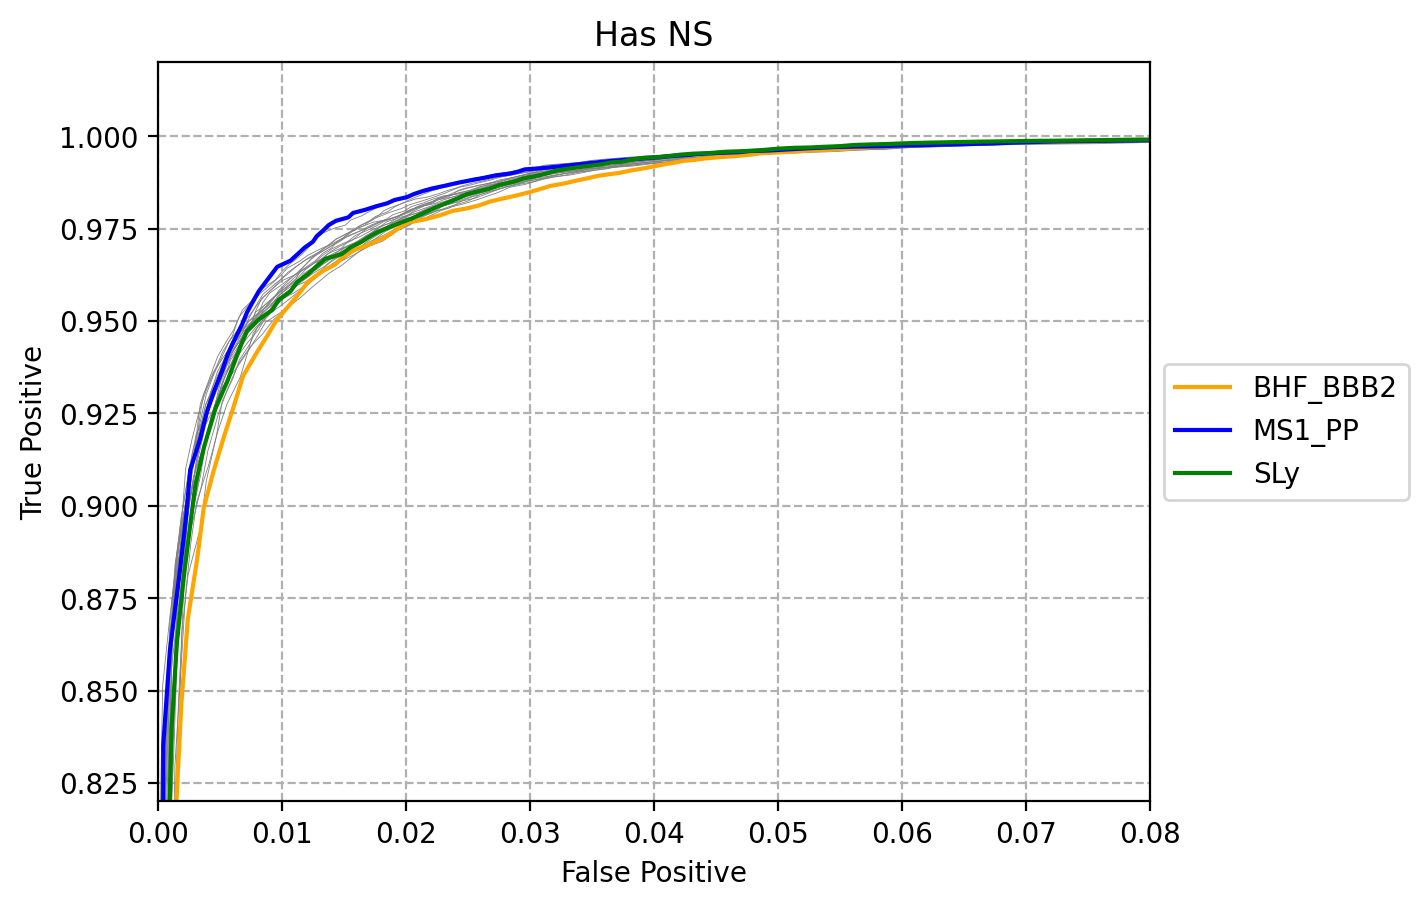
\includegraphics[width=0.45\textwidth]{/figs/HasNS_roc}
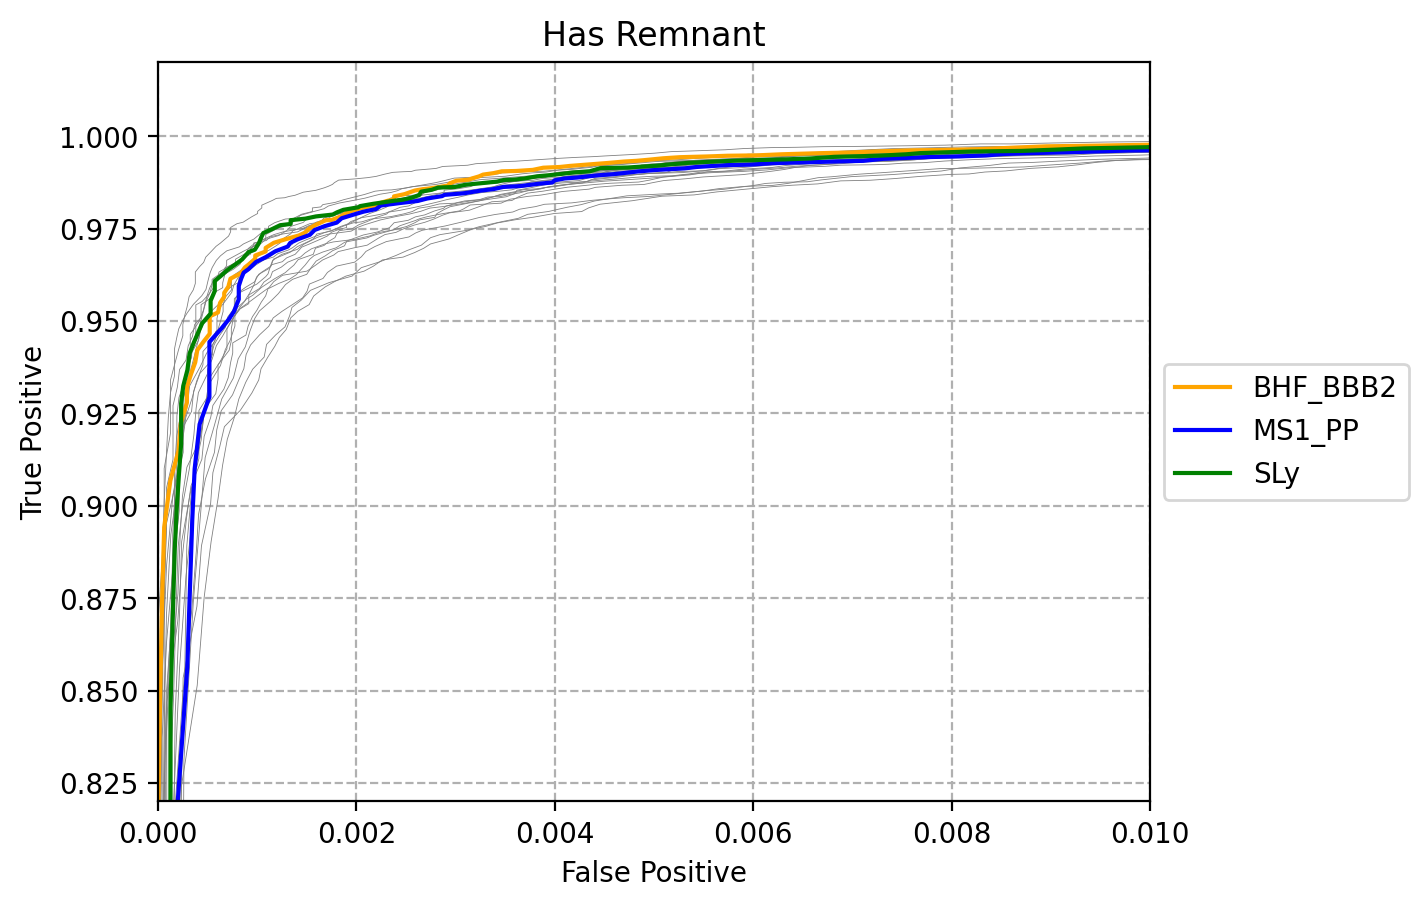
\includegraphics[width=0.45\textwidth]{/figs/HasREM_roc}
\caption{\label{fig:RF_roc} ROC curves}
\end{figure}

\begin{figure}
\centering
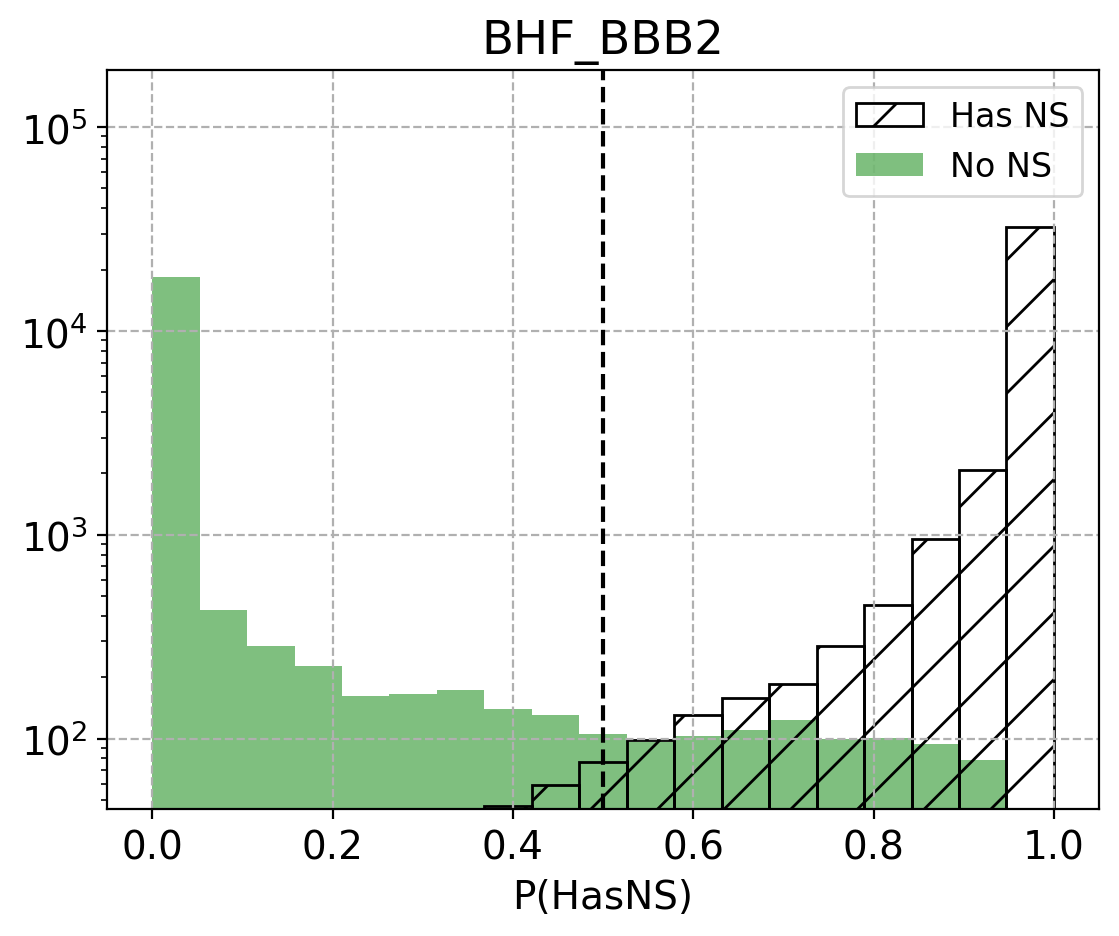
\includegraphics[width=0.45\textwidth]{/figs/BHF_BBB2_NShist}
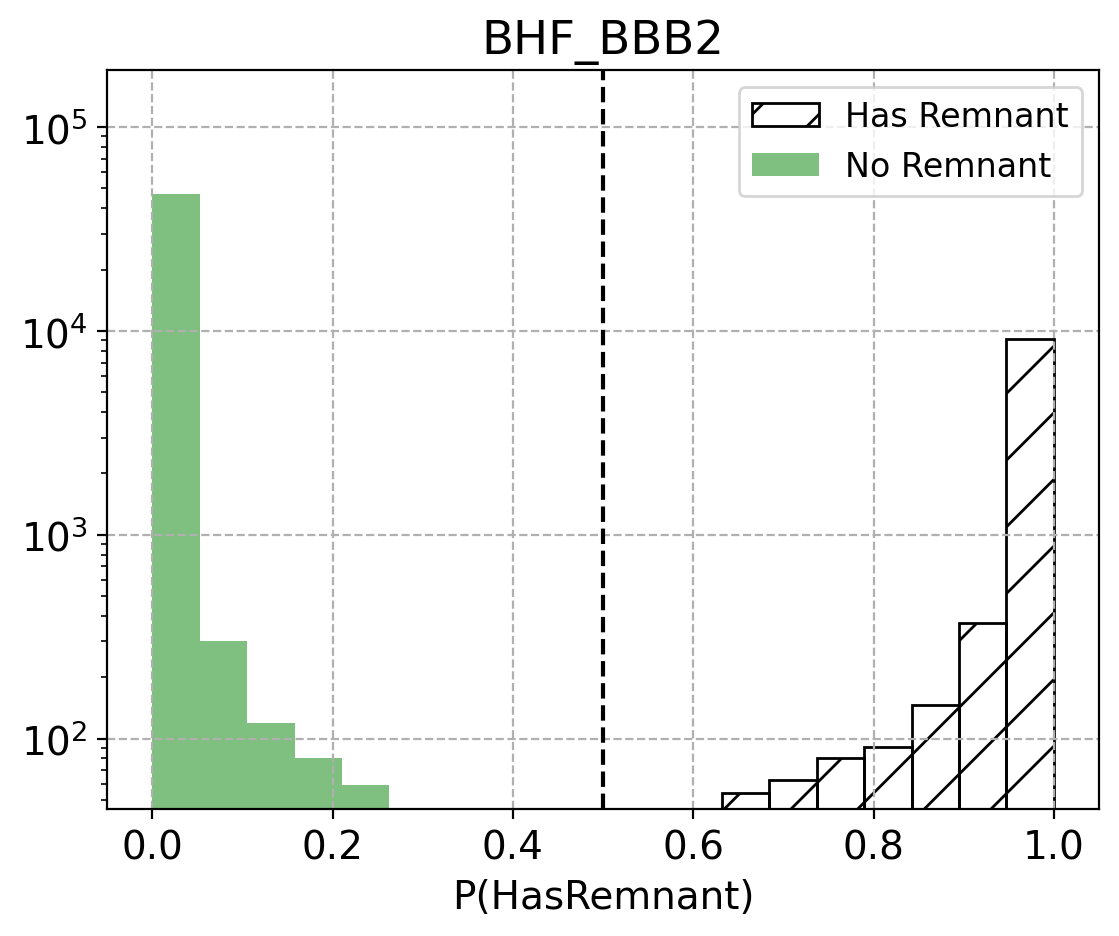
\includegraphics[width=0.45\textwidth]{/figs/BHF_BBB2_REMhist}
\caption{\label{fig:RF_hist_BHFBBB2} Histograms BHF BBB2}
\end{figure}

\begin{figure}
\centering
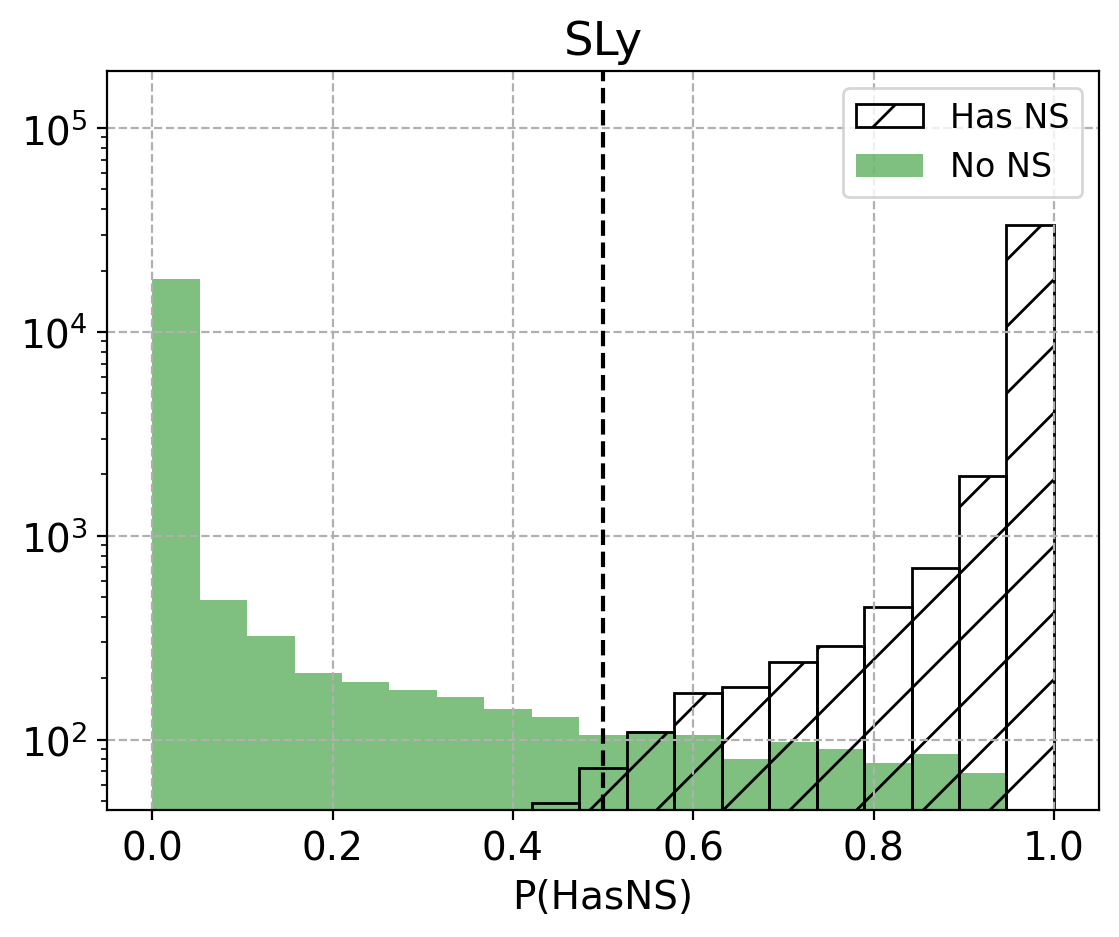
\includegraphics[width=0.45\textwidth]{/figs/SLy_NShist}
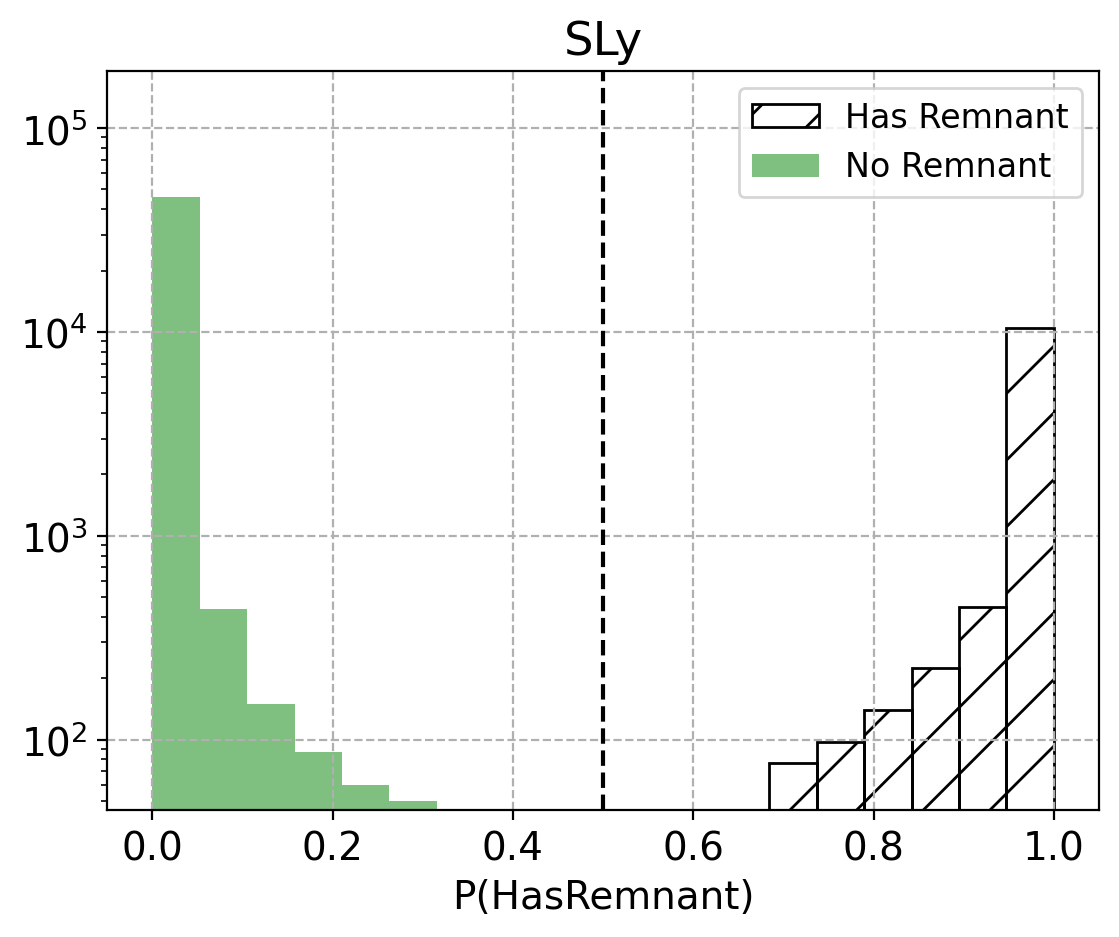
\includegraphics[width=0.45\textwidth]{/figs/SLy_REMhist}
\caption{\label{fig:RF_hist_SLY} Histograms SLy}
\end{figure}

\begin{figure}
\centering
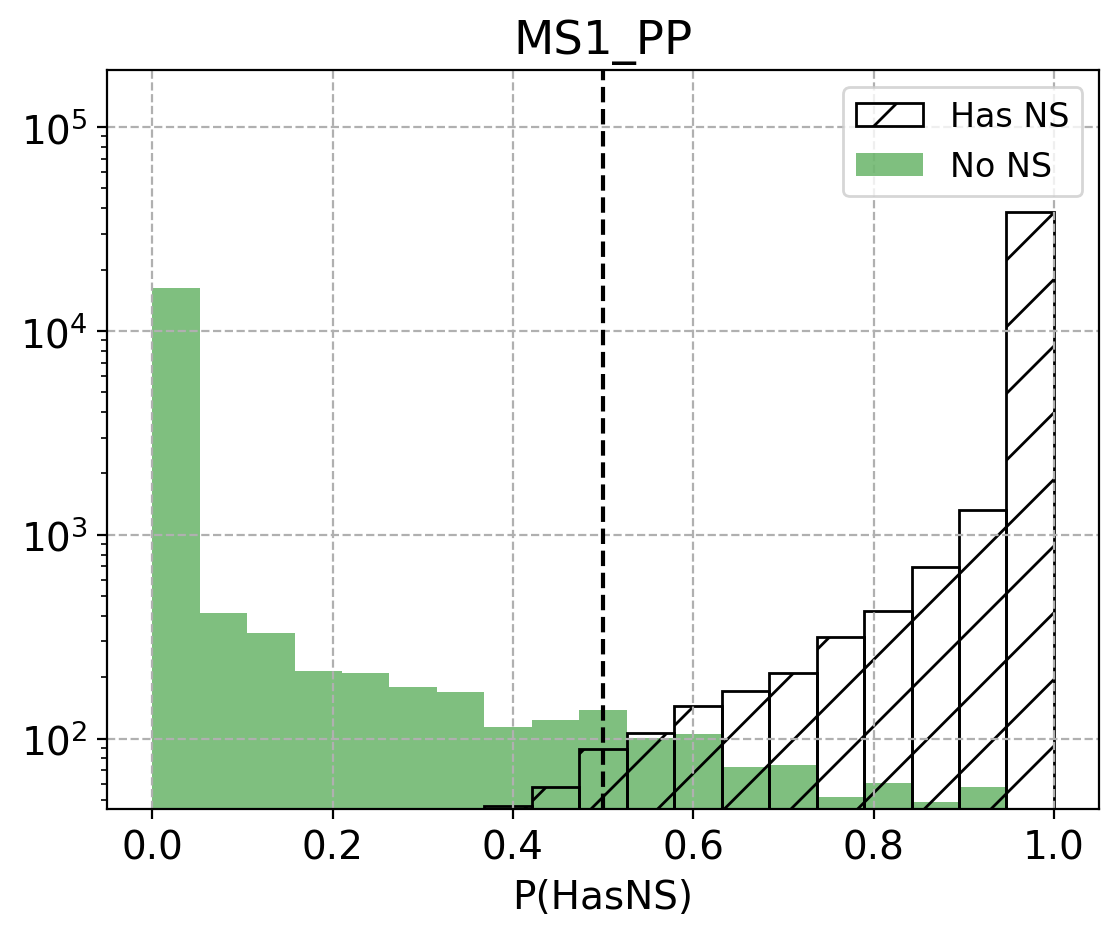
\includegraphics[width=0.45\textwidth]{/figs/MS1_PP_NShist}
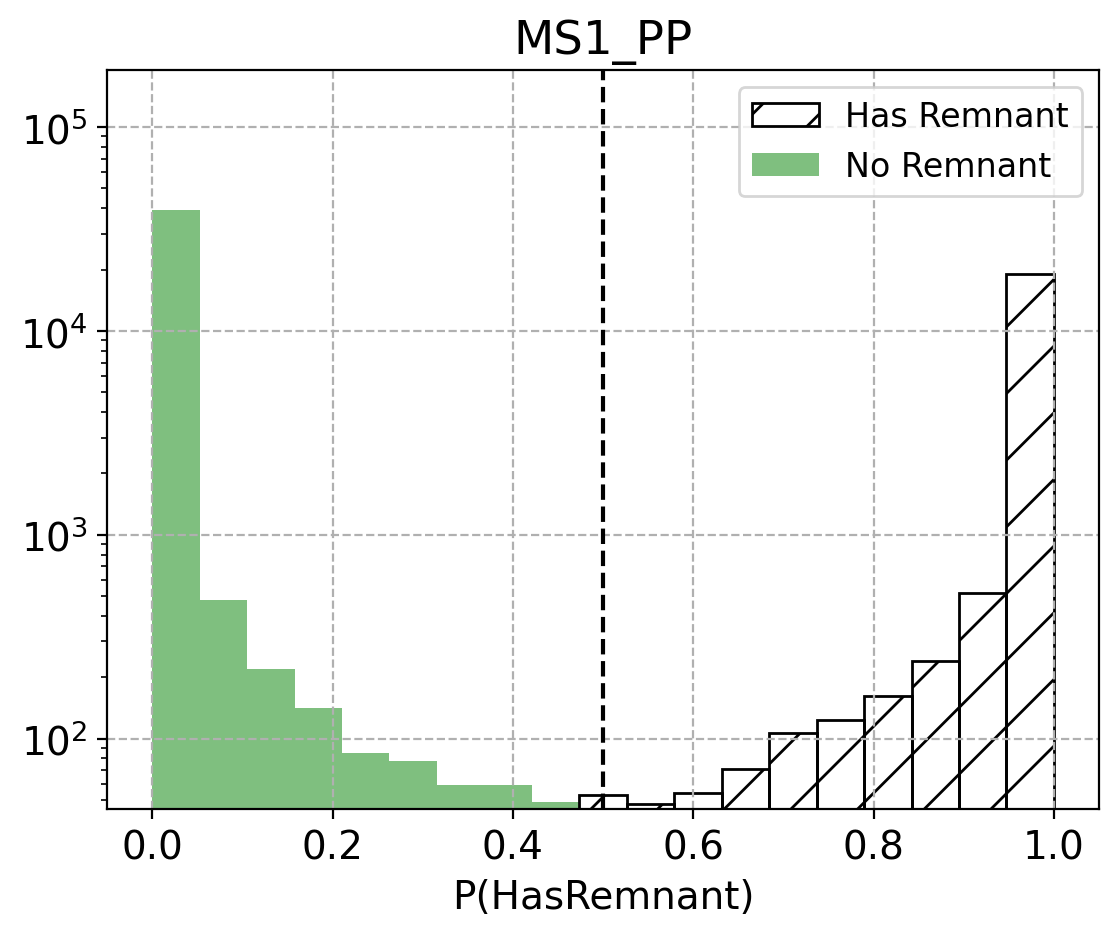
\includegraphics[width=0.45\textwidth]{/figs/MS1_PP_REMhist}
\caption{\label{fig:RF_hist_MS1PP} Histograms MS1 PP}
\end{figure}


 %plots and comments
%\input{GP_Results.tex}


%In order to decide which method gives a better performance in classifying this kind of events, we can apply them over testing data and finally do a comparison between both. A way to see how data is classified we can construct histograms where the number of events that are classified with a label (\texttt{HasNS/HasRemnant}) \texttt{True} or \texttt{False} will change with a given threshold of the probability. For an algorithm with perfect performance, all the events with label \texttt{True (False)} should be at \textit{p}(\texttt{label}) = 1 (\textit{p}(\texttt{label}) = 0).

%Another way to check the algorithm's performance is by building the so-called \textit{Receiver Operating Characteristic (ROC) Curve}. They show the variation of the true-positive rate (or efficiency) with the false-positive rate given a certain threshold for the probability. An algorithm with a proper performance will give a steeper ROC curve, or in other words, will have a higher eficiency with a lower false-positive rate.  


%In the ROC curves that we will present in the following subsections, we highlight three reference EoS in color, from which we show results in more detail. We select BHF\_BBB2 because is the model that give the lowest maximum mass, MS1\_PP as the model with the bigger maximum mass, and we also include SLy because is the most accepted EoS for NS modeling (reference), and is the one that was used in the injections that are our dataset.


%\subsection{Algorithm comparison}


%Here we talk about overall results and specifically from each algorithm in the
%subsections below.  \mmt{[MMT: Below I described how to check the performance of the algorithms. Maybe a table with all the scores/sensitivities/precisions from both %KNN and RF would be useful (already got it in a google doc)]}

%\mmt{To measure the performance of the classifiers we use some common statistical quantities.  The score is the number of correctly predicted events over the number %of total events (a perfect classifier has a score of 1).  It works best when there is an equal number of events for each label in the training set. It does not %consider the importance of misclassification, or that the training data can be biased towards one specific label.}

%\mmt{The mean score is computed by training the algorithm on the $90\%$ of the dataset and testing it on the remaining $10\%$, cycling the train/test combination over %the full dataset. To do that, we are going to use the training dataset, since it's the larger one.  In order to train and test the model and create the different %plots, we are going to use the training and testing files. }

%\mmt{Another useful quantity is the sensitivity. It is the ratio between the true positives and the sum of the true positives and false negatives.  It measures how %much the algorithm predicts \textit{true} (in our case it would be that the event has NS or has REM), when it is actually \textit{true}.Having a sensitivity equal to %1 would mean that our method predicts \textit{true} for every event. Therefore, a method with high sensitivity will barely miss true alarms. }

%\mmt{A quantity that measures how much you can trust a method when it predicts \textit{true} is the precision.  It is the ratio between the true positives and the %some of the true  and the false positives. A precision equal to 1 means that the method never predicts \textit{true} when it is actually \textit{false}. This means %that the method will never give false alarms. }

%\mmt{Finally, the F1 score $F1 = 2(\rm{precision \times sensitivity})/(\rm{precision+sensitivity})$ is a type of score that takes into consideration how precision and %sensitivity compensate each other. A perfect classifier would have a F1 score of 1.}

%To compare quantitatively the results from RF and KNN we compute the true positive and false positive rate for several threshold values, for both HasNS and HasREM, for the three selected EoS. These are tables \ref{tab:TPbhf}, \ref{tab:TPms1} and \ref{tab:TPsly}. For HasNS the two algorithms perform similarly, with almost the same TP for all threshold values and accross EoSs, although the false positive is smaller always in the RF. For HasREM we obtain that RF performs better than KNN in every case, with not only a smaller false positive rate, but a greater true positive rate.

%\begin{table}[]
%\centering
%\begin{tabular}{@{}c|cccc|cccc@{}}
%\toprule
%\multicolumn{1}{l|}{}          & \multicolumn{4}{c|}{Has NS}                       & \multicolumn{4}{c}{Has REM}                      \\ \midrule
%                               & \multicolumn{2}{c}{RF} & \multicolumn{2}{c|}{KNN} & \multicolumn{2}{c}{RF} & \multicolumn{2}{c}{KNN} \\
%\multicolumn{1}{l|}{Threshold} & TP         & FP        & TP          & FP         & TP         & FP        & TP         & FP         \\ \midrule
%0.1                            & 0.999      & 0.107     &   0.999          &  0.156          & 0.998      & 0.011     &    0.992        &  0.051          \\
%0.3                            & 0.998      & 0.068     &   0.996        &  0.117          & 0.993      & 0.005     &   0.974         &  0.017          \\
%0.5                            & 0.994      & 0.042     &   0.991          &  0.088           & 0.985      & 0.003     &   0.937         &  0.006          \\
%0.8                            & 0.967      & 0.014     &   0.966          & 0.043            & 0.957      & 0.001     &  0.845          &   0.001         \\ %\bottomrule
%\end{tabular}
%\caption{BHF\_BB2}
%\label{tab:TPbhf}
%\end{table}

